\documentclass[a4paper, 11pt, twoside]{jreport}
% include
\usepackage{gra_yasuda}
\usepackage{lscape}
\usepackage{graphicx}
\usepackage{here}
\usepackage{color}
\usepackage{amsmath}
\usepackage{subfig}
\usepackage{tascmac}
\usepackage{url}
\usepackage{ascmac}
\usepackage{booktabs}
\usepackage{otf}
\usepackage{comment}



%タイトル
\title{心理的効果を用いた人間とエージェントの繰り返し交渉戦略}
\etitle{Repetitive negotiation strategy of human and agent \\ using psychological effect}

%名前
\author{松下 昌悟}
\eauthor{Shogo MATSUSHITA}

%入学年度
\enteryear{2017}
%卒業年度
\graduateyear{2018}

%学籍番号
\studentnumber{17268508}

%提出日
\date{平成30年1月31日}

\begin{document}

%ここで行ピッチを指定
%フォントを変えるとサイズがリセットされてしまうので注意
\setlength{\baselineskip}{8truemm}

\renewcommand{\include}[1]{}
\renewcommand\documentclass[2][]{}

\maketitle

% ここにそれぞれのファイルを順番に並べる
% 目次や表目次、図目次も全部自動で作ってくれる
% 参照のために変更した時は3回くらいタイプセットすること

% 章立ては各自で適宜設定してください
\documentclass[a4paper, 10.5pt, twoside]{jreport}

% include
\usepackage{gra_yasuda}
\usepackage{lscape}
\usepackage{graphicx}
\usepackage{here}
\usepackage{color}
\usepackage{amsmath}
\usepackage{subfig}
\usepackage{tascmac}
\usepackage{url}
\usepackage{ascmac}
\usepackage{booktabs}
\usepackage{otf}
\usepackage{comment}



%タイトル
\title{心理的効果を用いた人間とエージェントの繰り返し交渉戦略}
\etitle{Repetitive negotiation strategy of human and agent \\ using psychological effect}

%名前
\author{松下 昌悟}
\eauthor{Shogo MATSUSHITA}

%入学年度
\enteryear{2017}
%卒業年度
\graduateyear{2018}

%学籍番号
\studentnumber{17268508}

%提出日
\date{平成30年1月31日}

\begin{document}

%ここで行ピッチを指定
%フォントを変えるとサイズがリセットされてしまうので注意
\setlength{\baselineskip}{8truemm}


%ここから内容

% Chapter 1
\chapter{はじめに}\label{cha:1}

\section{背景}
交渉スキルは友人への頼みごと等の日常的な小規模な問題だけでなく企業の提携,国家間の取引等の大規模な問題を解決する際に必要である.
特に,組織的な団体に属する場合は目標を達成するために交渉を行う必要がある場面が多い.
しかし,交渉スキルなどの対人能力は大学を卒業した学生であっても不十分であり\cite{graduate},交渉スキルの不足により不利益を被ることも多い.
交渉スキルを高めるには専門家による指導を受け,体験学習で実践を行う必要があり,受講の費用も高額であるため習得コストが非常に高い.
このように交渉スキルを高めるためのコストは非常に高いが,教育ツールとして交渉エージェントを包含したソフトウェアを用いることで習得にかかるコストを劇的に削減することができる.また,専門家による指導は指導者と受講者の時間的制約もあるが,ソフトウェアによる指導の場合は時間的制約も削減することが可能である.
人間とエージェントの交渉において交渉における5つの原則\cite{nego_principle}のうち3つをどの程度達成しているかを数値化し視覚化する研究\cite{visualize}も行われており,教育ツールへの応用が期待されている.
交渉はビジネス,衝突解消,AIなど複数の分野で研究されているが,前述のように交渉スキルを教育するためのツールなどへ応用が可能であるため,人間とエージェントとの交渉への関心が高まっている\cite{vr}.

近年,行動科学の研究では交渉中に感情が与える影響に関心が高まってきている\cite{behavior}.
感情は重要な社会的機能を有しており,個人の信条,欲望,意図などの情報を伝達する.
例として多くの研究では交渉において怒りは相手からより多くの譲歩を引き出す一方で,喜びは相手からあまり譲歩を引き出すことができないという結果が示されている\cite{angryhappy}.
したがって,交渉相手が怒った場合は,合意に達するために要求を下げ,一方で,交渉相手が喜んだ場合は,戦略的に多くの要求をすることができる.
これらの心理的効果が人間同士の交渉だけではなく人間とエージェントの交渉でも同様な効果があることが示された\cite{emotion}.
このように,人間とエージェントが交渉を行う際も感情などの心理的効果が交渉結果に影響を与えるが,人間とエージェントの交渉ではこれらの影響を考慮していないモデルが多かった.
その要因として,エージェント同士の交渉に用いるエージェントを作成するプラットフォームとしてGenius\cite{genius}などがある一方で,人間と交渉可能なエージェントを作成するために最適なプラットフォームがないという問題点があった.
複数論点交渉問題について扱うColored Trails\cite{ct},Colored TrailsのWEB版であるWebCT\cite{webct},自然言語による交渉に焦点を当てたNegoChat\cite{negochat}などが存在しているが,これらのプラットフォームは単一のチャネルを用いたコミュニケーションに重点を置いており,感情に関する情報を表出するチャネルが含まれていない.
人間と交渉を行うことができるエージェントを作成するためのプラットフォームであるIAGO\cite{iago}は感情やメッセージの送信を行うためのチャネルがあらかじめ用意されており,IAGOが登場してからは,心理的効果を反映したエージェントに関する研究が増えつつある.一方で,繰り返し交渉に対応できる戦略が少ないのが現状である.


また,作成したエージェントを用いて交渉を行い,個人効用や社会的余剰の値を競い合う自動交渉エージェント競技会(Automated Negotiation Agent Competition(ANAC))が2010年から毎年開催されている\cite{anac2010-2015,anac2016,anac2017,anac2018}.
ANACでは2016年まではエージェント同士の交渉を行うリーグのみが開催されていたが,自動交渉はDiplomacyなどの交渉を行うゲームAIや人間との交渉に応用されることが期待されており,ANACでは2017年からDiplomacyを取り扱うDiplomacy Strategy Game League,人間とエージェントが交渉を行うHuman-Agent Negotiation Leagueが開催された.Human-Agent Negotiation Leagueではエージェントを作成するためのプラットフォームとしてIAGOが採用されており,2018年からは繰り返し交渉を取り扱っており,繰り返し交渉に対応した戦略に対する関心が高まってきている.

\section{本研究の目的}
本研究では,人間と交渉を行うことが可能でかつ同じ相手と繰り返し交渉する際に個人効用が高くなるようなエージェントを提案することを目的とする.
具体的には,交渉時間の増加,交渉回数の増加に応じて相手の提案を受諾する水準を変化させることで繰り返し交渉に対応する.
本研究では,提案を受諾する水準を変化させる手法として人間の心理的効果を利用した交渉術である段階的要請法および譲歩的要請法に着目し,
これらの手法を組み合わせて人間とエージェントの自動交渉に用いることで,繰り返し交渉に対応可能な戦略を提案する.
また,提案手法およびIAGOのベースラインのエージェントと人間が交渉を行う実験を実施し評価を行うことで,提案手法の有効性を示すことを目的とする.

\section{本論文の構成}
以下に本論文の構成を述べる.第2章では,関連研究として,自動交渉エージェント競技会の概要,IAGOの概要,心理的効果が交渉に与える影響についての研究について述べる.
第3章では,本研究で取り扱う交渉問題である複数論点交渉問題と繰り返し交渉問題について述べる.
第4章では,提案手法の詳細として,段階的要請法および譲歩的要請法とこれらを組み合わせた繰り返し戦略について述べる.
第5章では,繰り返し戦略に用いるパラメータを決定するために行なった予備実験の結果について述べる.
第6章では,予備実験で決定したパラメータを用いて被験者に対して行なった評価実験の結果について述べる.
最後に,第7章では本研究のまとめと今後の課題を示す.

%内容ここまで

\chapter*{謝辞}
本論文を執筆するにあたり,多数の方々からご指導・ご協力いただきましたことを,心より御礼申し上げます.

指導教員である藤田桂英准教授には,研究の機会を与えていただき,研究の方針に関する助言や発表練習等の
多大なるご指導や助言をいただきましたことを深く感謝いたします.

研究に関する知識のご教示に加えて,本実験の準備を行うにあたってWEBサーバを構築する際にお力添えいただいた松根鷹生様に深く感謝申し上げます.
また,藤田桂英研究室の皆様には研究に必要な知識や意見等をいただいたことを心より感謝いたします.

本実験を行うにあたってお忙しい中ご協力いただいた同期の編入生の方々,および安井貴規様がいなければ本論文は完成に至りませんでした.
心より御礼申し上げます.

最後に,様々な面で私を支えていただいた家族に,心より感謝いたします.ありがとうございました.

\bibliographystyle{plain}
\bibliography{reference}


\begin{comment}
%付録で発表論文をつけてアピールだ!!

\renewcommand{\bibname}{付録 発表論文一覧}
%\chapter{発表論文一覧}

\begin{thebibliography}{99}
\item S. Kakimoto and K. Fujita. 二者間複数論点交渉問題におけるパレートフロント推定手法の提案. Joint Agent Workshop and Symposium, 2014.
\item S. Kakimoto and K. Fujita. Estimating Pareto Fronts using Interdependency between Issues for Bilateral Multi-issue Closed Nonlinear Negotiations. Applications Knowledge and Service Technology for Life, Environment, and Sustainability workshop(KASTLES),2014.
\item S. Kakimoto and K. Fujita. 二者間非線形交渉問題におけるパレートフロント推定を利用した自動交渉エージェントの設計と評価. 情報処理学会 第177回 知能システム研究会, 2014.

\end{thebibliography}

\end{comment}

\end{document}


\documentclass[a4paper, 10.5pt, twoside]{jreport}

% include
\usepackage{gra_yasuda}
\usepackage{lscape}
\usepackage{graphicx}
\usepackage{here}
\usepackage{color}
\usepackage{amsmath}
\usepackage{subfig}
\usepackage{tascmac}
\usepackage{url}
\usepackage{ascmac}
\usepackage{booktabs}
\usepackage{otf}
\usepackage{comment}



%タイトル
\title{心理的効果を用いた人間とエージェントの繰り返し交渉戦略}
\etitle{Repetitive negotiation strategy of human and agent \\ using psychological effect}

%名前
\author{松下 昌悟}
\eauthor{Shogo MATSUSHITA}

%入学年度
\enteryear{2017}
%卒業年度
\graduateyear{2018}

%学籍番号
\studentnumber{17268508}

%提出日
\date{平成30年1月31日}

\begin{document}

%ここで行ピッチを指定
%フォントを変えるとサイズがリセットされてしまうので注意
\setlength{\baselineskip}{8truemm}


%ここから内容

% Chapter 2
\chapter{関連研究}\label{cha:2}

\section{自動交渉エージェント競技会(ANAC)}

\subsection{ANAC}
自動交渉エージェント競技会(Automated Negotiation Agent Competition)は各自が作成したエージェント同士で交渉を行い個人獲得効用や社会的余剰などを競う競技会である\cite{anac2010-2015,anac2016,anac2017,anac2018}.
ANACは毎年開催され,
2010年(第1回)から2016年(第7回)まではInternational Conference on Autonomous Agents and Multiagent Systems(AAMAS)と共催で行われた.
2017年(第8回),2018年(第9回)はInternational Joint Conference on Artificial Intelligence(IJCAI)と共催で行われ,
2019年度(第10回)もIJCAIと共催で行われる予定である.
ANACは以下の4点を目的としている.
\begin{itemize}
  \item 未知の相手に対し,様々な状況で巧みに交渉できる実用的な交渉エージェントの設計を促進
  する
  \item 様々な交渉戦略を客観的に評価する指標を提供する
  \item 様々な学習手法,適応戦略,交渉相手のモデル構築を探求する
  \item 最先端の交渉エージェントと交渉シナリオを収集し,研究コミュニティに提供する
\end{itemize}

ANACでは2016年までは自動交渉のプラットフォームであるGeniusを用いて単一のリーグが開催されていた.
2017年からは複数のリーグが開催され,Geniusを使用し任意のドメインで交渉を行うRepeated Multilateral Negotiation League,Bandana(BAsic eNvironment for Diplomacy playing Automated Negotiating Agents)を使用しボードゲームのDiplomacyの交渉を扱うDiplomacy
Strategy Game League,IAGO(Interactive Arbitration Guide Online)を使用し
人間とエージェントの交渉を扱うHuman-Agent Negotiation Leagueの3つのリーグが開催された.
また,2018年からはHuman-Agent Negotiation Leagueでは人間とエージェントの繰り返し交渉が行われている.


\begin{figure}[tb]
  \centering
  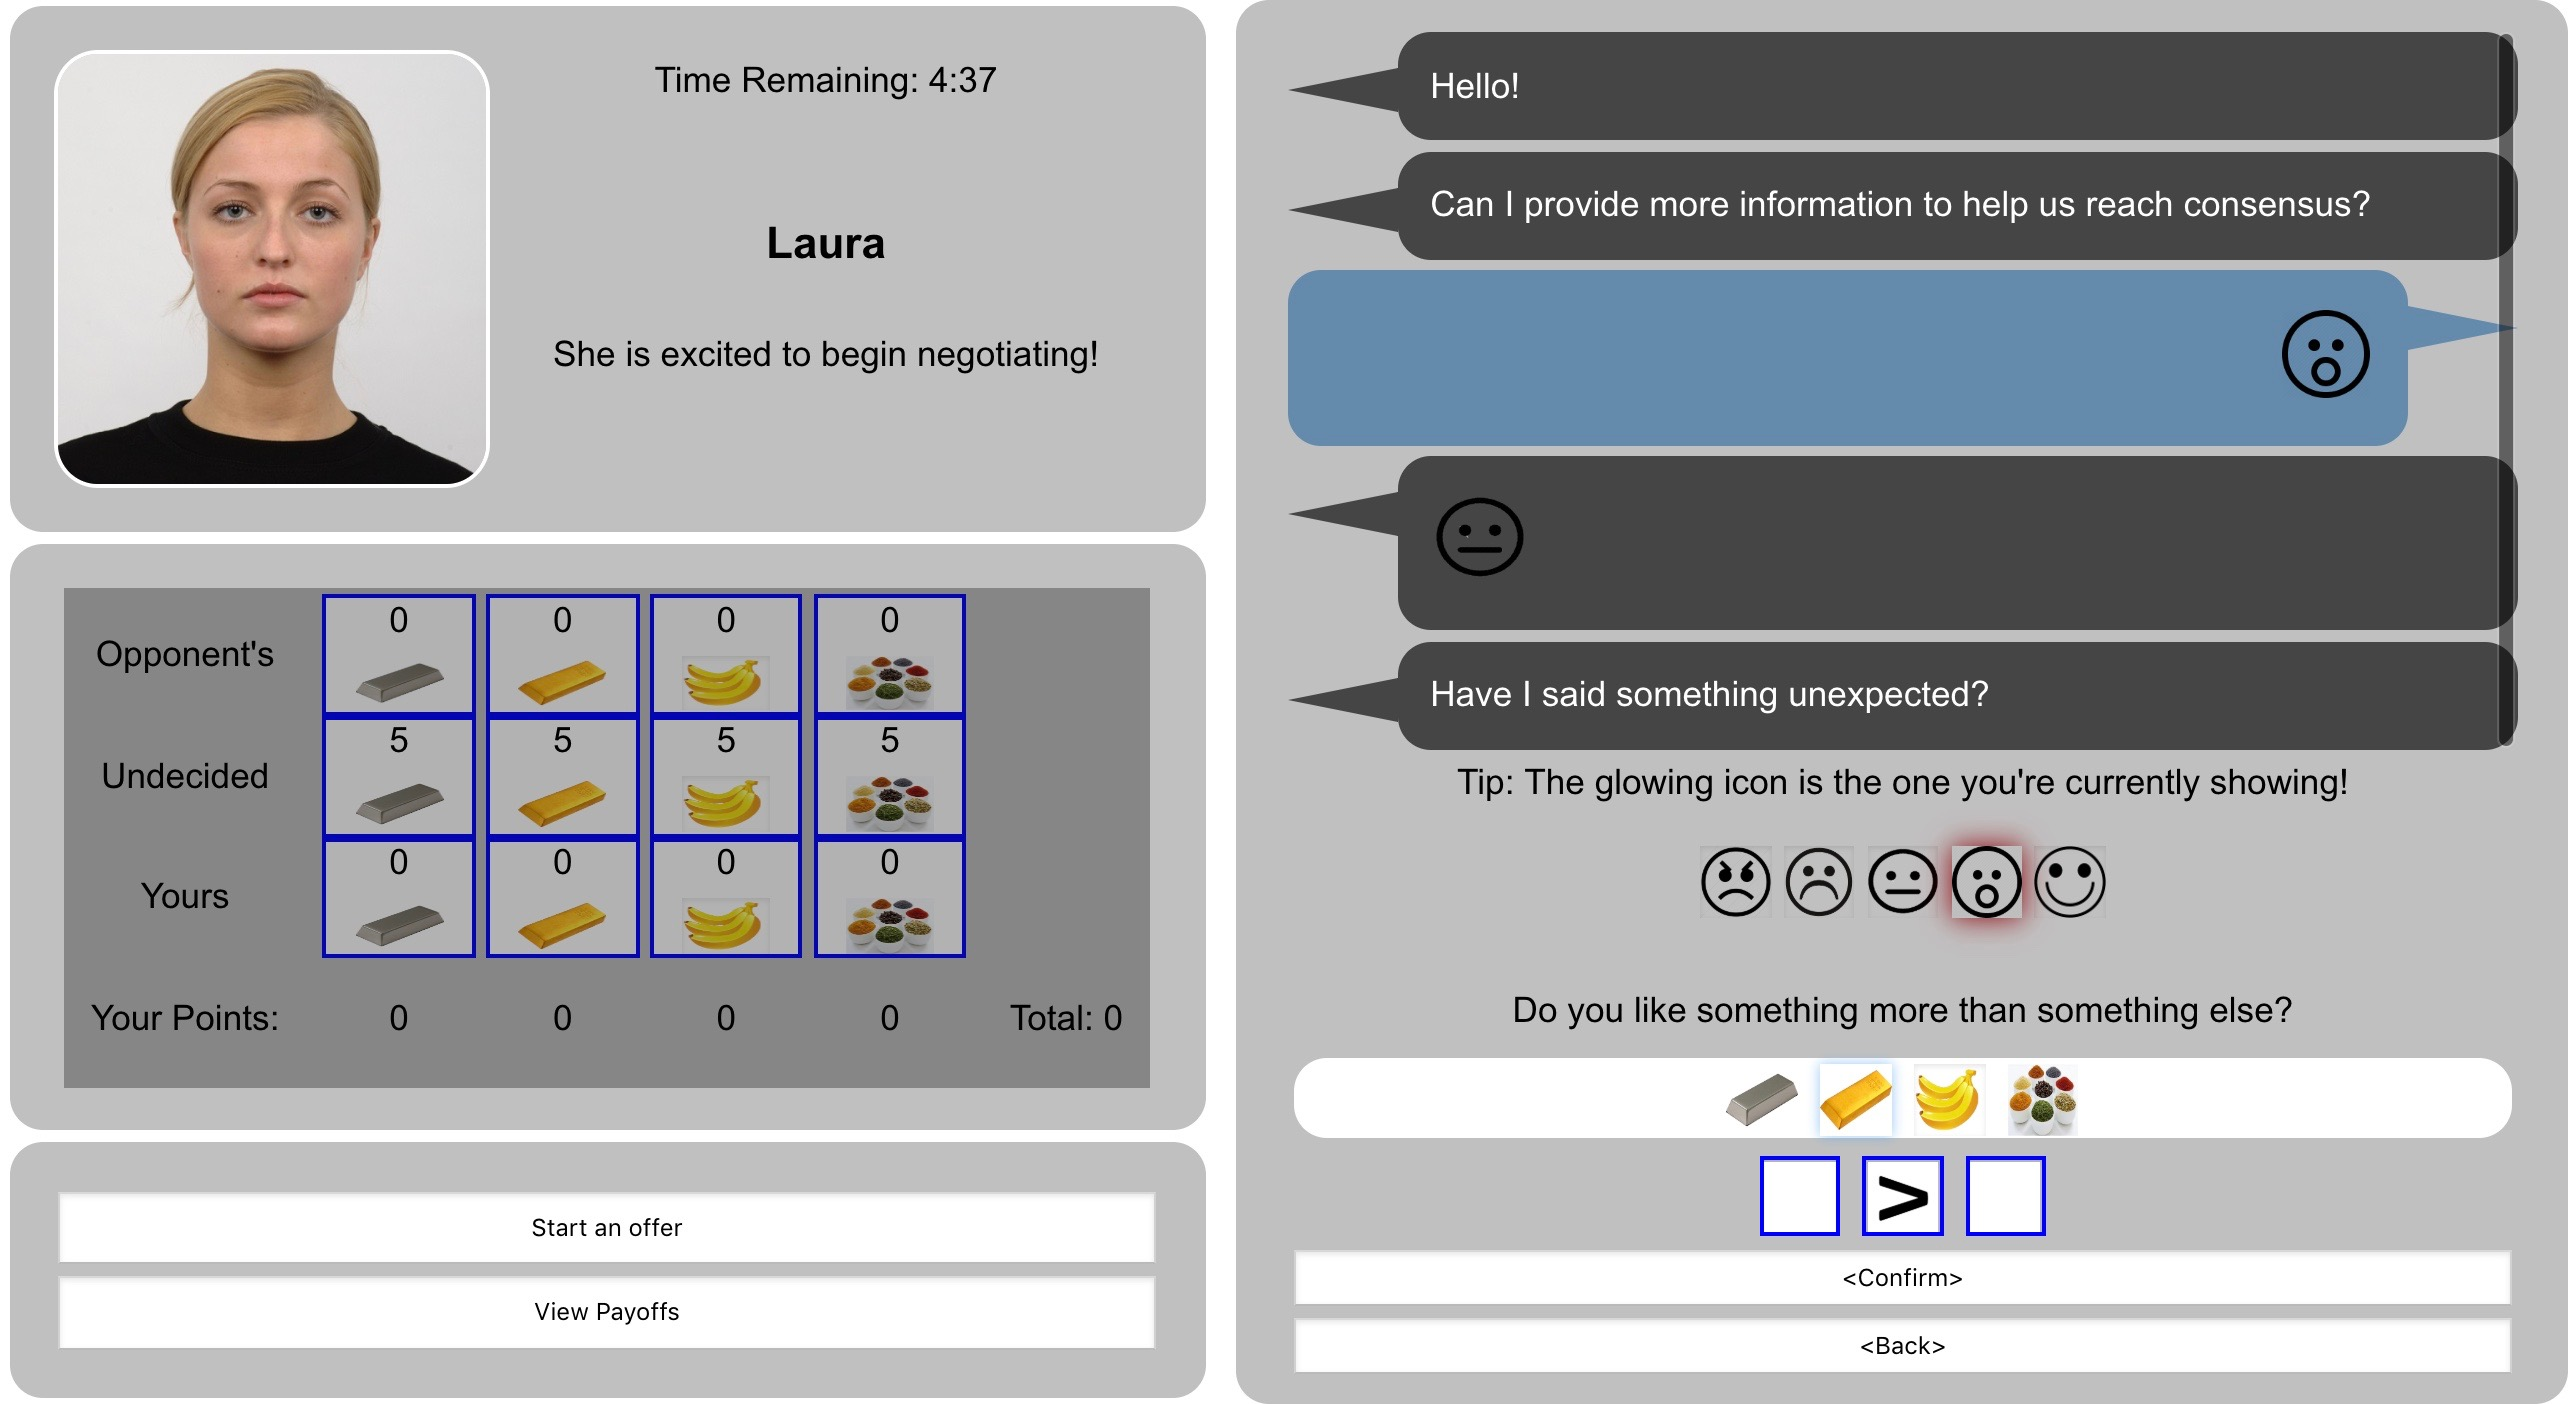
\includegraphics[width=15truecm]{image/IAGO.eps}
  \caption{IAGOのインタフェース}
  \label{fig:iago}
\end{figure}

\subsection{IAGO}
IAGO(Interactive Arbitration Guide Online)はANACのHuman-Agent Negotiationリーグで使用される自動交渉のプラットフォームである\cite{iago}.
IAGOのインタフェースを図\ref{fig:iago}に示す.
IAGOでは,人間と交渉を行うエージェントおよび交渉のドメインを作成することが可能である.IAGOの特徴として以下の3点が挙げられる\cite{pinocchio}.

\begin{enumerate}
  \item WEB上で動作する
  \item APIが公開されている
  \item 人間同士の交渉で用いられるチャネルが利用可能
\end{enumerate}

第1の特徴により,エージェントと交渉を行うクライアントはWEBブラウザ上で交渉を行うことが可能である.
したがって,クライアントはソフトウェアのインストールなどを行うことなく交渉を開始することができる.
第2の特徴により,競技会や研究のためのエージェントおよび交渉ドメインの設計を容易に行うことが可能となる.
第3の特徴により,エージェントおよびクライアントは感情の表出,メッセージの送信,選好の公開および誘発などを交渉中に行うことが可能となる.
これにより,人間同士の交渉で用いられるチャネルによる交渉結果への影響を研究することおよび
これらのチャネルを利用した交渉を行うエージェントを作成することが容易となる.
IAGOでは,サンプルとしてPinocchioエージェントがあらかじめ用意されており,本研究では,Pinocchioエージェントをベースにして戦略の実装し,実験を行う.

\section{自動交渉における心理的効果に関する研究}
人間とエージェントの交渉における心理的効果に関する研究としてCelsoらの研究がある\cite{emotion}.
この研究では,交渉相手がエージェントだと知らされた上で感情が交渉に対して影響を与えるか調査している.
同時に,感情の伝達方法によって交渉に与える効果の差異についても調査している.
交渉はAlternating Offers Protocol\cite{aop}を用いて行い,感情は怒り,喜び,中立の3種類,感情の伝達方法は言語,画像の2種類について実験を行なっている.
実験は150人の被験者に対して行われ,
実験の結果,エージェントが怒りの感情を相手に伝えた場合被験者は大きく譲歩し,喜びの感情を相手に伝えた場合被験者はあまり譲歩しないという結果となった.
また,感情の伝達方法については譲歩の度合いに有意差はなく,感情は伝達方法とは独立に交渉結果に影響を与え,感情によって交渉結果が異なることが明らかになった.
この研究では,今後の展望として繰り返し交渉において感情のような心理的効果が与える影響について調査する必要性について述べられている.

%内容ここまで

\chapter*{謝辞}
本論文を執筆するにあたり,多数の方々からご指導・ご協力いただきましたことを,心より御礼申し上げます.

指導教員である藤田桂英准教授には,研究の機会を与えていただき,研究の方針に関する助言や発表練習等の
多大なるご指導や助言をいただきましたことを深く感謝いたします.

研究に関する知識のご教示に加えて,本実験の準備を行うにあたってWEBサーバを構築する際にお力添えいただいた松根鷹生様に深く感謝申し上げます.
また,藤田桂英研究室の皆様には研究に必要な知識や意見等をいただいたことを心より感謝いたします.

本実験を行うにあたってお忙しい中ご協力いただいた同期の編入生の方々,および安井貴規様がいなければ本論文は完成に至りませんでした.
心より御礼申し上げます.

最後に,様々な面で私を支えていただいた家族に,心より感謝いたします.ありがとうございました.

\bibliographystyle{plain}
\bibliography{reference}


\begin{comment}
%付録で発表論文をつけてアピールだ!!

\renewcommand{\bibname}{付録 発表論文一覧}
%\chapter{発表論文一覧}

\begin{thebibliography}{99}
\item S. Kakimoto and K. Fujita. 二者間複数論点交渉問題におけるパレートフロント推定手法の提案. Joint Agent Workshop and Symposium, 2014.
\item S. Kakimoto and K. Fujita. Estimating Pareto Fronts using Interdependency between Issues for Bilateral Multi-issue Closed Nonlinear Negotiations. Applications Knowledge and Service Technology for Life, Environment, and Sustainability workshop(KASTLES),2014.
\item S. Kakimoto and K. Fujita. 二者間非線形交渉問題におけるパレートフロント推定を利用した自動交渉エージェントの設計と評価. 情報処理学会 第177回 知能システム研究会, 2014.

\end{thebibliography}

\end{comment}

\end{document}


\documentclass[a4paper, 10.5pt, twoside]{jreport}

% include
\usepackage{gra_yasuda}
\usepackage{lscape}
\usepackage{graphicx}
\usepackage{here}
\usepackage{color}
\usepackage{amsmath}
\usepackage{subfig}
\usepackage{tascmac}
\usepackage{url}
\usepackage{ascmac}
\usepackage{booktabs}
\usepackage{otf}
\usepackage{comment}



%タイトル
\title{心理的効果を用いた人間とエージェントの繰り返し交渉戦略}
\etitle{Repetitive negotiation strategy of human and agent \\ using psychological effect}

%名前
\author{松下 昌悟}
\eauthor{Shogo MATSUSHITA}

%入学年度
\enteryear{2017}
%卒業年度
\graduateyear{2018}

%学籍番号
\studentnumber{17268508}

%提出日
\date{平成30年1月31日}

\begin{document}

%ここで行ピッチを指定
%フォントを変えるとサイズがリセットされてしまうので注意
\setlength{\baselineskip}{8truemm}

%ここから内容

% Chapter 1
\chapter{問題設定}\label{cha:1}

\section{複数論点交渉問題}
本研究では,交渉問題の中でも論点が複数存在する複数論点交渉問題を扱う.エージェント$A_1$と$A_2$が交渉を行う場合を考える.エージェント$a \in \{ A_1, A_2 \}$の目的関数$f$は,$a$の効用関数$U_{a}$と全ての合意案候補集合$S$を用いると式\ref{eq:objectFunc}と表すことができる.
\begin{equation}
  f = \argmax_{s \in S} U_{a}(s)
  \label{eq:objectFunc}
\end{equation}

複数論点交渉問題の場合,目的関数$g$は式\ref{eq:socialSurplus}で表され,この目的関数の値は社会的余剰と呼ばれる.
\begin{equation}
  g = \argmax_{s \in S} \sum_{a \in \{ A_1, A_2 \}} U_{a}(s)
  \label{eq:socialSurplus}
\end{equation}

一つの交渉問題はそれぞれドメインと呼ばれ,論点数$N$のドメインは固有の論点集合$I = \{ i_1, i_2, ..., i_N \}$を持つ.
また,論点$i_k \in I$は選択肢集合$V_k = \{ v_{k1}, v_{k2}, ... ,v_{kn_k} \}$を持つ.ただし,論点$i_k$の選択肢数を$n_k$と定義する.

各論点$i_k \in I$についてそれぞれ選択肢$v_k \in V_k$を一つずつ選んだものを合意案候補(Bid)と呼び,
$s = (v_1, v_2, ..., v_N)$ として表現される.また,全ての合意案候補集合$S$は式\ref{eq:Bid}と表すことができる.
\begin{equation}
  S = \{ s = (v_1, v_2, ..., v_N) \, | \, v_k \in V_k , 1 \leqq k \geqq N \}
  \label{eq:Bid}
\end{equation}

エージェントは各論点$i_k$について重み$w_k$$(\sum_{k = 1}^N w_k = 1)$および選択肢の評価値$eval(v_k \in V_k)$を持つ.
ただし,$eval(v_k \in V_k)$は最大値が1となるように正規化されているものとする.このとき,エージェントの効用関数$U$は式\ref{eq:Utility}となる.
\begin{equation}
  U(s) = \sum_{k = 1}^N w_k \cdot eval(v_k)
  \label{eq:Utility}
\end{equation}
また,各エージェントに対し留保価格(reservation value) 設定される場合がある.
留保価格は合意形成に失敗した際にエージェントが獲得できる効用値である.

\section{繰り返し交渉問題}
本研究では,繰り返し交渉問題を扱う.繰り返し交渉問題は,交渉問題の中でエージェント$A_1$と$A_2$が複数回交渉を行うものを指す.
本研究では,繰り返し交渉問題の中でも特に,以下の2つの関係を満たす交渉問題について取り扱う.
\begin{enumerate}
  \item 各交渉において各論点における各選択肢の一番高い値をエージェント$A_1$が選択した場合の効用$U_1$と$A_2$が選択した場合の効用$U_2$は等しい
  \item $1,2, \cdots n$回目の交渉において$U_1$および$U_2$の値は不変である
\end{enumerate}
エージェント$a = \{ A_1, A_2 \}$にとっての論点$i_k$についての選択肢の実際の価値を$val(v_{ak} \in V_{ak})$とすると,
各交渉におけるエージェント$A_1$と$A_2$の効用値の関係は式\ref{eq:bothUtility}となる.
\begin{equation}
  \sum_{k = 1}^N w_{A_1k} \cdot val(v_{A_1k}) = \sum_{k = 1}^N w_{A_2k} \cdot val(v_{A_2k})
  \label{eq:bothUtility}
\end{equation}

また,$n$回目の交渉におけるエージェント$a = \{ A_1, A_2 \}$にとっての論点$i_k$についての重みを$w_{A_1k}^n$選択肢の実際の価値を$val(v_{ak}^n \in V_{ak}^n)$とすると,$1,2, \cdots ,n$回目の交渉における効用値の関係は式\ref{eq:repeatedUtility}となる.
\begin{equation}
  \sum_{k = 1}^N w_{ak}^1 \cdot val(v_{ak}^1) = \sum_{k = 1}^N w_{ak}^2 \cdot val(v_{ak}^2) = \cdots = \sum_{k = 1}^N w_{ak}^n \cdot val(v_{ak}^n)
  \label{eq:repeatedUtility}
\end{equation}


%内容ここまで

\chapter*{謝辞}
本論文を執筆するにあたり,多数の方々からご指導・ご協力いただきましたことを,心より御礼申し上げます.

指導教員である藤田桂英准教授には,研究の機会を与えていただき,研究の方針に関する助言や発表練習等の
多大なるご指導や助言をいただきましたことを深く感謝いたします.

研究に関する知識のご教示に加えて,本実験の準備を行うにあたってWEBサーバを構築する際にお力添えいただいた松根鷹生様に深く感謝申し上げます.
また,藤田桂英研究室の皆様には研究に必要な知識や意見等をいただいたことを心より感謝いたします.

本実験を行うにあたってお忙しい中ご協力いただいた同期の編入生の方々,および安井貴規様がいなければ本論文は完成に至りませんでした.
心より御礼申し上げます.

最後に,様々な面で私を支えていただいた家族に,心より感謝いたします.ありがとうございました.

\bibliographystyle{plain}
\bibliography{reference}


\begin{comment}
%付録で発表論文をつけてアピールだ!!

\renewcommand{\bibname}{付録 発表論文一覧}
%\chapter{発表論文一覧}

\begin{thebibliography}{99}
\item S. Kakimoto and K. Fujita. 二者間複数論点交渉問題におけるパレートフロント推定手法の提案. Joint Agent Workshop and Symposium, 2014.
\item S. Kakimoto and K. Fujita. Estimating Pareto Fronts using Interdependency between Issues for Bilateral Multi-issue Closed Nonlinear Negotiations. Applications Knowledge and Service Technology for Life, Environment, and Sustainability workshop(KASTLES),2014.
\item S. Kakimoto and K. Fujita. 二者間非線形交渉問題におけるパレートフロント推定を利用した自動交渉エージェントの設計と評価. 情報処理学会 第177回 知能システム研究会, 2014.

\end{thebibliography}

\end{comment}

\end{document}


\documentclass[a4paper, 10.5pt, twoside]{jreport}

% include
\usepackage{gra_yasuda}
\usepackage{lscape}
\usepackage{graphicx}
\usepackage{here}
\usepackage{color}
\usepackage{amsmath}
\usepackage{subfig}
\usepackage{tascmac}
\usepackage{url}
\usepackage{ascmac}
\usepackage{booktabs}
\usepackage{otf}
\usepackage{comment}



%タイトル
\title{心理的効果を用いた人間とエージェントの繰り返し交渉戦略}
\etitle{Repetitive negotiation strategy of human and agent \\ using psychological effect}

%名前
\author{松下 昌悟}
\eauthor{Shogo MATSUSHITA}

%入学年度
\enteryear{2017}
%卒業年度
\graduateyear{2018}

%学籍番号
\studentnumber{17268508}

%提出日
\date{平成30年1月31日}

\begin{document}

%ここで行ピッチを指定
%フォントを変えるとサイズがリセットされてしまうので注意
\setlength{\baselineskip}{8truemm}


%ここから内容

% Chapter 3
\chapter{繰り返し交渉戦略の提案}\label{cha:3}

\section{段階的要請法(Foot-in-the-Door technique)}
段階的要請法は交渉の際に用いられる心理的手法である.
段階的要請法の概要を図\ref{fig:foot}に示す.
段階的要請法では,最初に相手に対して小さい要求を行い,徐々に要求を上げていく手法である.
この手法は自分の行動を一貫したものにしたいという人間の一貫性の原理を利用した交渉術である.

図\ref{fig:foot}では売り手は買い手に対して話を聞いてもらうという小さな要求を行い,
次にこの要求を承諾した買い手に対して商品を購入してもらうという大きな要求を行なっている.
このように,段階的要請法では事前に小さな要求を相手に承諾させることで真の要求を相手に拒否させづらくさせることが可能である.

\begin{figure}[h]
  \centering
  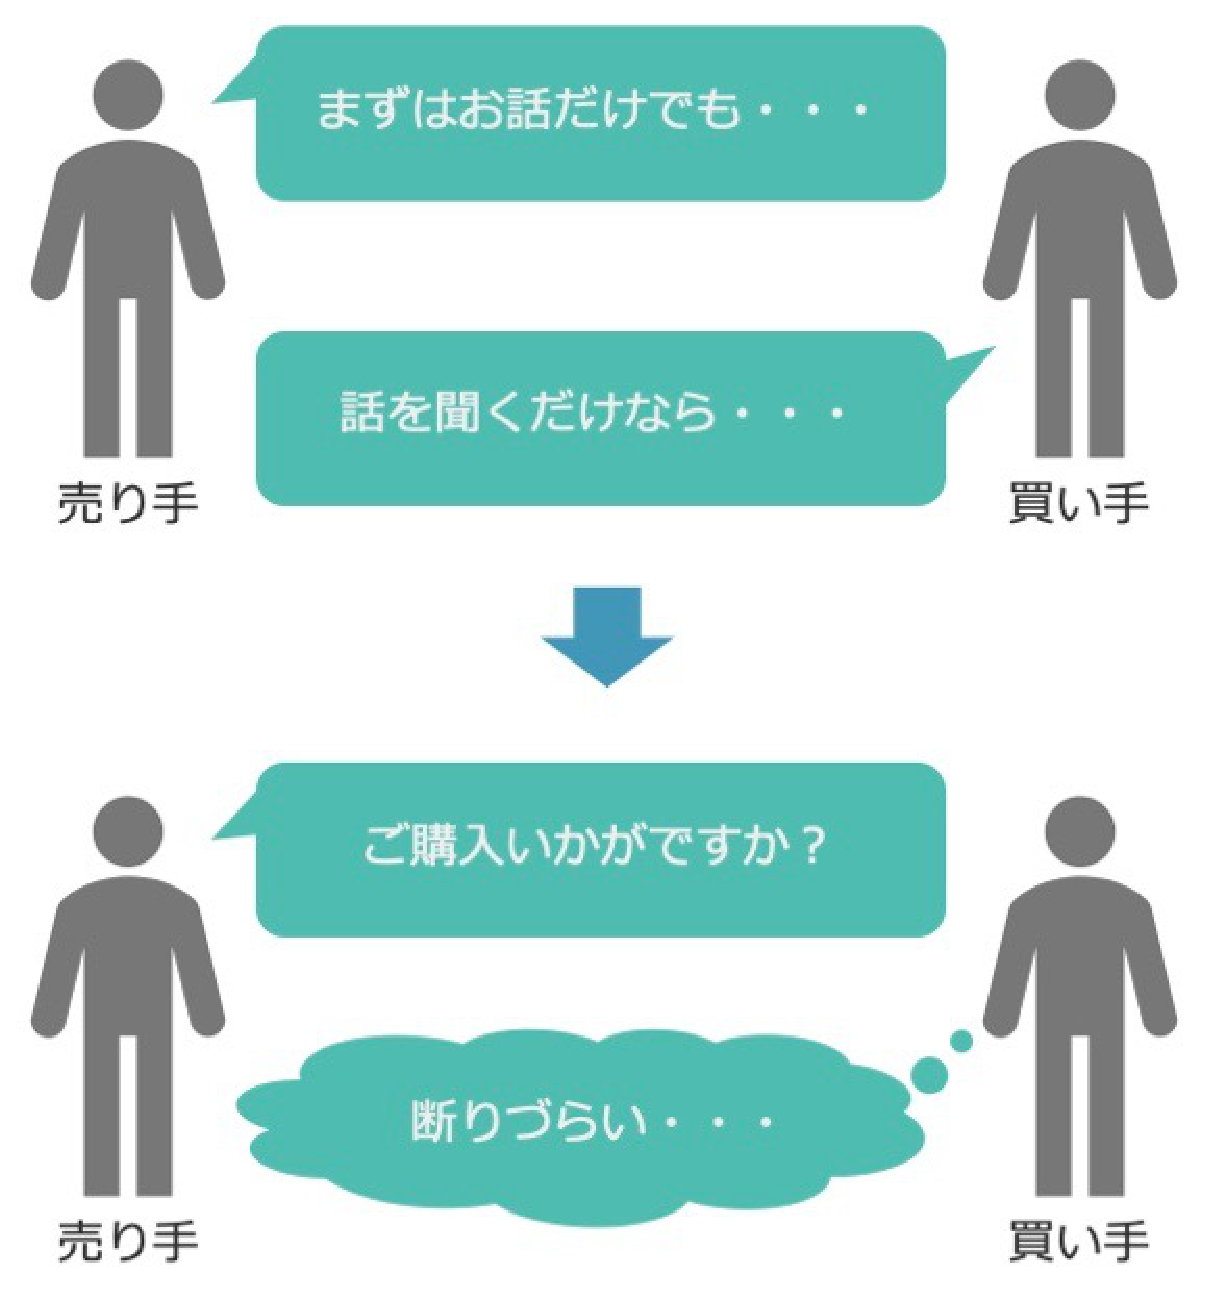
\includegraphics[width=10truecm]{image/foot.eps}
  \caption{段階的要請法の概要}
  \label{fig:foot}
\end{figure}

\section{譲歩的要請法(Door-in-the-Face technique)}

譲歩的要請法は交渉の際に用いられる心理的手法である.
譲歩的要請法の概要を図\ref{fig:door}に示す.
譲歩的要請法では,段階的要請法とは対照的に最初に相手に対して大きい要求を行い,徐々に要求を下げていく手法である.
この手法は相手が譲歩してきたため自分も譲歩した方が良いという人間の返報性の原理を利用した交渉術である.

図\ref{fig:door}では売り手は買い手に対して3万円で商品を買ってもらうという大きな要求を行い,
次にこの要求を拒否した買い手に対して商品を値下げし2万円で商品を買ってもらうという小さな要求を行なっている.
このように,譲歩的要請法では事前に大きな要求を行い,相手に要求を拒否させることで真の要求を相手に拒否させづらくさせることが可能である.

\begin{figure}[h]
  \centering
  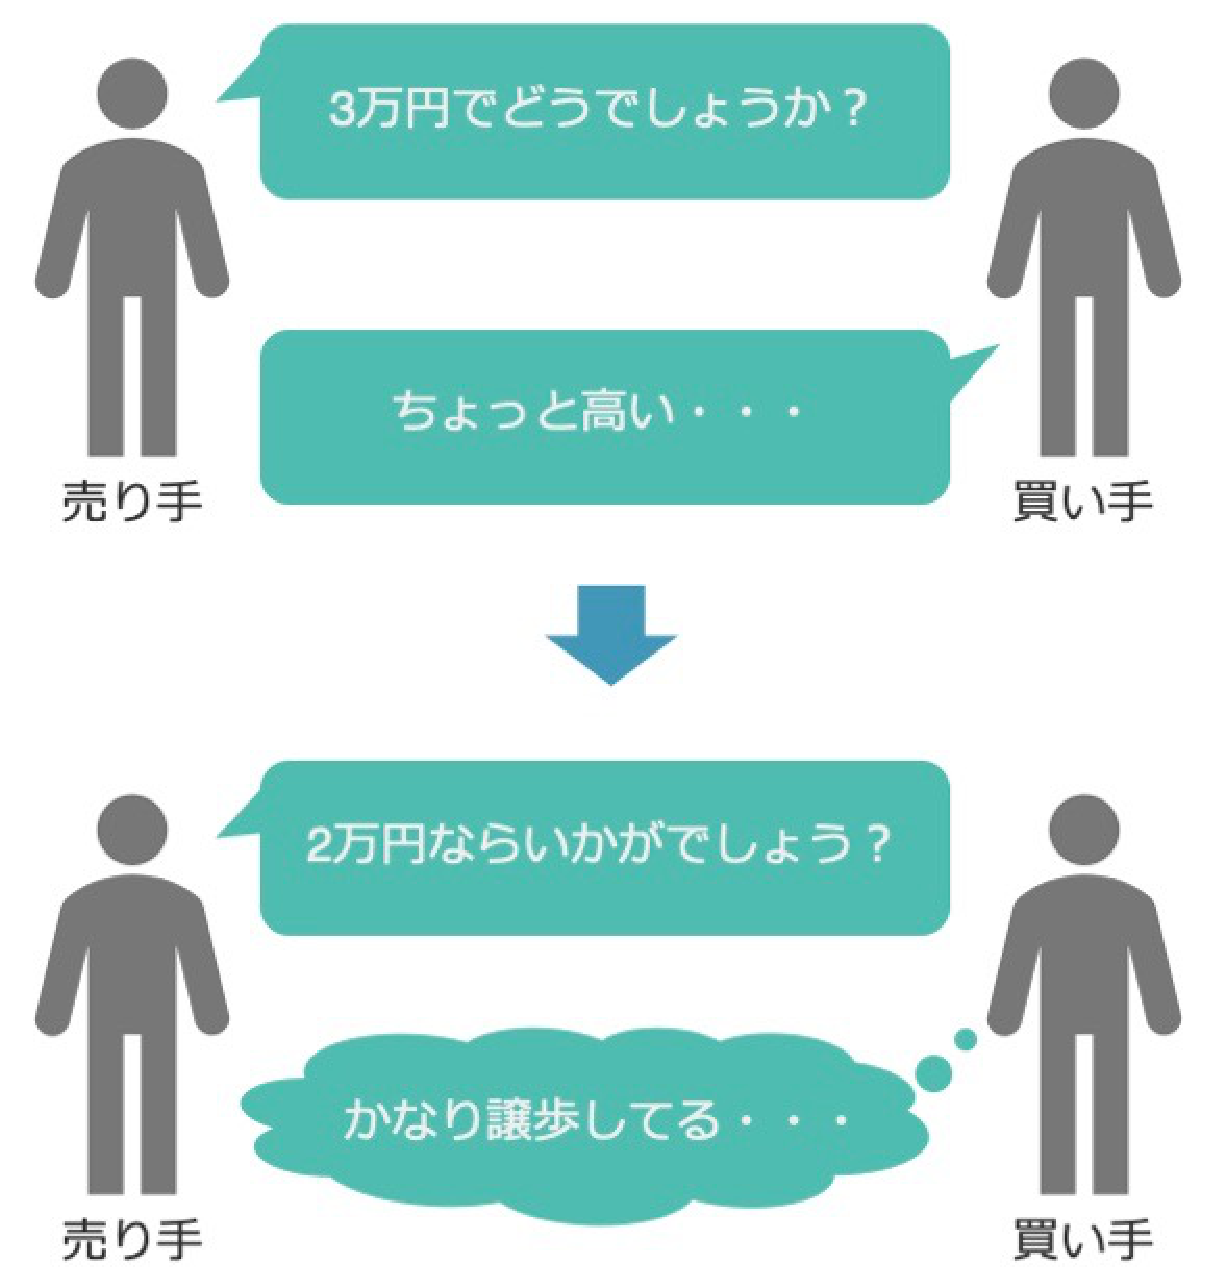
\includegraphics[width=10truecm]{image/door.eps}
  \caption{譲歩的要請法の概要}
  \label{fig:door}
\end{figure}

\section{段階的要請法と譲歩的要請法を組み合わせた交渉戦略の提案}

本稿では,先述した段階的要請法と譲歩的要請法を組み合わせることで繰り返し交渉に対応した戦略を提案する.
提案手法の概要を図\ref{fig:propose}に示す.

提案手法では相手の提案を受諾する水準を変化させる.1回の交渉ごとでは,時間経過に伴って水準を変化させる.
すなわち,図\ref{fig:propose}のように交渉開始時の水準が\mathrm{L}であった場合,時間経過によって水準を\mathrm{L\pm \alpha}に変化させる.以下,この水準を内側の水準と記述する.
また,同時に交渉回数の増加に伴って水準を変化させる.
すなわち,図\ref{fig:propose}のように1回目の交渉開始時の水準が\mathrm{L}であった場合,2回目の交渉開始時の水準を\mathrm{L\pm \meta}に変化させる.以下,この水準外側の水準と記述する.

\begin{figure}[h]
  \centering
  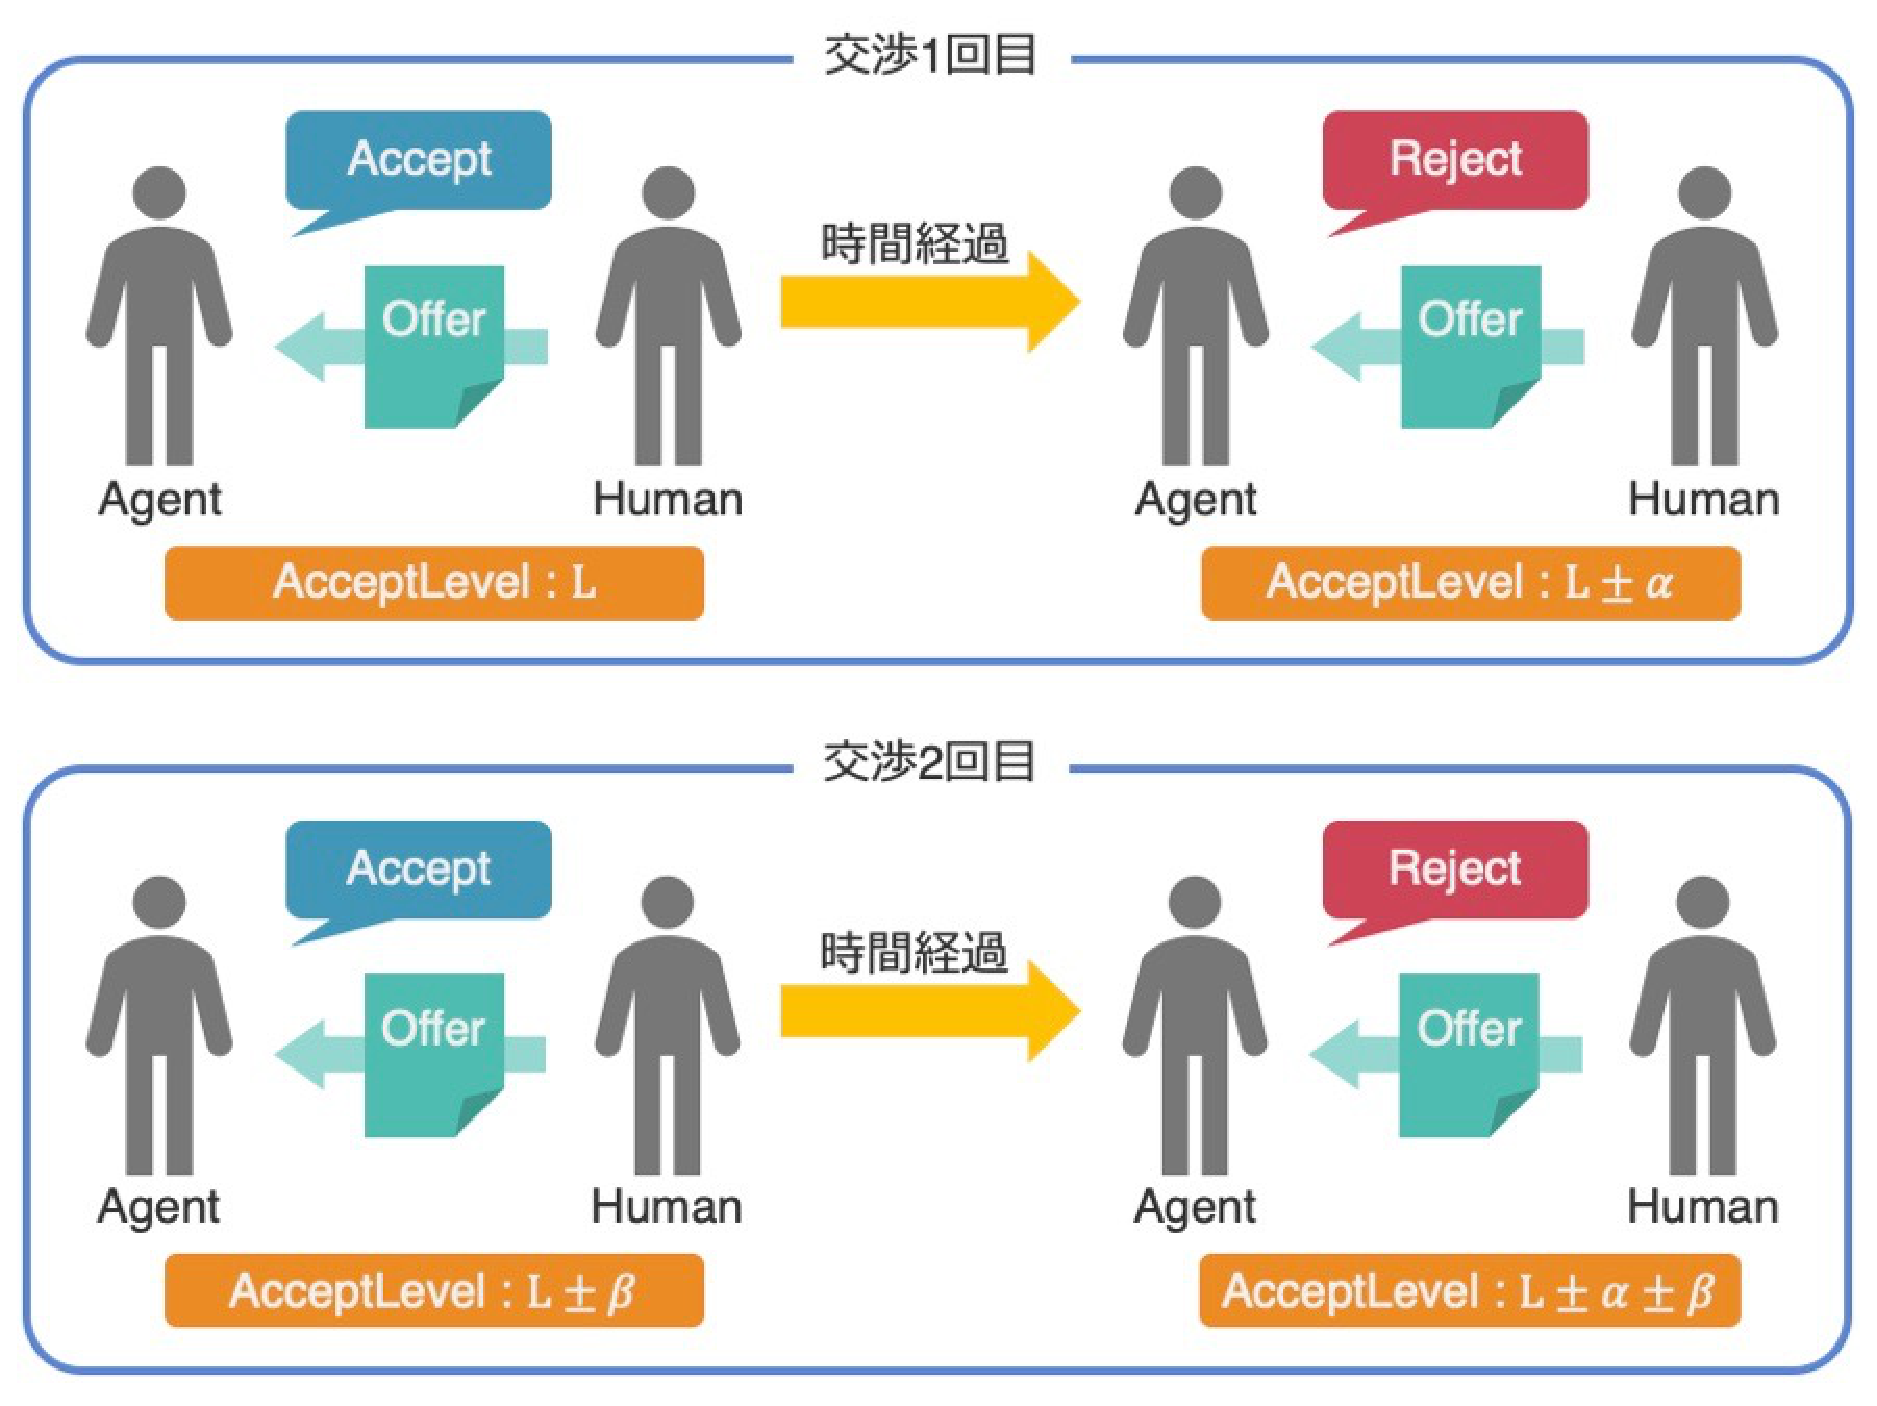
\includegraphics[width=15truecm]{image/propose.eps}
  \caption{提案手法の概要}
  \label{fig:propose}
\end{figure}

提案手法では,これら2種類の水準の変化を組み合わせることで,繰り返し交渉に対応する.
水準の変化にそれぞれ段階的要請法,譲歩的要請法,水準を変化させない方法の3種類を適用した9種類の戦略を用意する.
戦略の組み合わせと対応する戦略名を表\ref{tab:strategy}に示す.
表\ref{tab:strategy}の9種の戦略の内,内側および外側の戦略がどちらも変化しないNotNotはベースラインとして使用し,NotNotを除外した8種類の戦略を提案手法とし,第4章の予備実験および第5章の評価実験を行う.

\begin{table}[htb]
  \begin{center}
    \caption{戦略の組み合わせ}
    \label{tab:strategy}
    \begin{tabular}{|c|c|c|c|c|} \hline
      戦略名 & 内側の戦略 & 外側の戦略 & \alpha の値 & \beta の値 \\ \hline \hline
      NotNot & \multirow{3}{*}{なし} & なし & \multirow{3}{*}{0} & 0 \\ \cline{1-1} \cline{3-3} \cline{5-5}
      NotFoot & & 段階的要請法 & & $> 0$ \\ \cline{1-1} \cline{3-3} \cline{5-5}
      NotDoor & & 譲歩的要請法 & & $< 0$ \\ \hline
      FootNot & \multirow{3}{*}{段階的要請法} & なし & \multirow{3}{*}{$> 0$} & 0 \\ \cline{1-1} \cline{3-3} \cline{5-5}
      FootFoot & & 段階的要請法 & & $> 0$ \\ \cline{1-1} \cline{3-3} \cline{5-5}
      FootDoor & & 譲歩的要請法 & & $< 0$ \\ \hline
      DoorNot & \multirow{3}{*}{譲歩的要請法} & なし & \multirow{3}{*}{$< 0$} & 0 \\ \cline{1-1} \cline{3-3} \cline{5-5}
      DoorFoot & & 段階的要請法 & & $> 0$ \\ \cline{1-1} \cline{3-3} \cline{5-5}
      DoorDoor & & 譲歩的要請法 & & $< 0$ \\ \hline
    \end{tabular}
  \end{center}
\end{table}

%内容ここまで

\chapter*{謝辞}
本論文を執筆するにあたり,多数の方々からご指導・ご協力いただきましたことを,心より御礼申し上げます.

指導教員である藤田桂英准教授には,研究の機会を与えていただき,研究の方針に関する助言や発表練習等の
多大なるご指導や助言をいただきましたことを深く感謝いたします.

研究に関する知識のご教示に加えて,本実験の準備を行うにあたってWEBサーバを構築する際にお力添えいただいた松根鷹生様に深く感謝申し上げます.
また,藤田桂英研究室の皆様には研究に必要な知識や意見等をいただいたことを心より感謝いたします.

本実験を行うにあたってお忙しい中ご協力いただいた同期の編入生の方々,および安井貴規様がいなければ本論文は完成に至りませんでした.
心より御礼申し上げます.

最後に,様々な面で私を支えていただいた家族に,心より感謝いたします.ありがとうございました.

\bibliographystyle{plain}
\bibliography{reference}


\begin{comment}
%付録で発表論文をつけてアピールだ!!

\renewcommand{\bibname}{付録 発表論文一覧}
%\chapter{発表論文一覧}

\begin{thebibliography}{99}
\item S. Kakimoto and K. Fujita. 二者間複数論点交渉問題におけるパレートフロント推定手法の提案. Joint Agent Workshop and Symposium, 2014.
\item S. Kakimoto and K. Fujita. Estimating Pareto Fronts using Interdependency between Issues for Bilateral Multi-issue Closed Nonlinear Negotiations. Applications Knowledge and Service Technology for Life, Environment, and Sustainability workshop(KASTLES),2014.
\item S. Kakimoto and K. Fujita. 二者間非線形交渉問題におけるパレートフロント推定を利用した自動交渉エージェントの設計と評価. 情報処理学会 第177回 知能システム研究会, 2014.

\end{thebibliography}

\end{comment}

\end{document}


\documentclass[a4paper, 10.5pt, twoside]{jreport}

% include
\usepackage{gra_yasuda}
\usepackage{lscape}
\usepackage{graphicx}
\usepackage{here}
\usepackage{color}
\usepackage{amsmath}
\usepackage{subfig}
\usepackage{tascmac}
\usepackage{url}
\usepackage{ascmac}
\usepackage{booktabs}
\usepackage{otf}
\usepackage{comment}



%タイトル
\title{心理的効果を用いた人間とエージェントの繰り返し交渉戦略}
\etitle{Repetitive negotiation strategy of human and agent \\ using psychological effect}

%名前
\author{松下 昌悟}
\eauthor{Shogo MATSUSHITA}

%入学年度
\enteryear{2017}
%卒業年度
\graduateyear{2018}

%学籍番号
\studentnumber{17268508}

%提出日
\date{平成30年1月31日}

\begin{document}

%ここで行ピッチを指定
%フォントを変えるとサイズがリセットされてしまうので注意
\setlength{\baselineskip}{8truemm}


%ここから内容

% Chapter 4
\chapter{予備実験}\label{cha:4}

\section{目的と概要}
提案手法に用いる各種パラメータを決定することを目的としてエージェント同士での交渉を行う実験を行う.
具体的には提案手法の戦略を適用した8つのエージェントと予備実験用の戦略を適用したエージェントでそれぞれ交渉を行う.
本実験では,提案手法の戦略を適用したエージェントの個人効用が高いほど良いパラメータであると評価する.

\section{実験設定}
本実験では,各論点が$0\sim 5$の計6つの選択肢を有する,4つの論点について交渉を行う.

本実験で用いるドメインの詳細およびパラメータを表\ref{tab:pre_domain},表\ref{tab:pre_para}にそれぞれ示す.

\begin{table}[htb]
  \begin{center}
    \caption{予備実験で用いるドメイン}
    \label{tab:pre_domain}
    \begin{tabular}{|c|c|c|c|} \hline
      論点数 & 各論点の選択肢数 & 繰り返し回数 & 留保価格 \\ \hline \hline
      4 & 6 & 5 & 4 \\ \hline
    \end{tabular}
  \end{center}
\end{table}

\begin{table}[htb]
  \begin{center}
    \caption{予備実験で用いるパラメータ}
    \label{tab:pre_para}
    \begin{tabular}{|c|c|c|c|c|c|} \hline
      & \alpha の初期値 & \alpha の増分 & \beta の初期値 & \beta の増分 & \alpha の更新回数 \\ \hline \hline
      取りうる値 & 0.0 \sim 8.0 & 0.5 \sim 4.0 & 0.0 \sim 8.0 & 0.5 \sim 4.0 & 1 \sim 10 \\ \hline
      刻み幅 & 1.0 & 0.5 & 1.0 & 0.5 & 1 \\ \hline
      取りうる値の総数 & 9 & 8 & 9 & 8 & 10 \\ \hline
    \end{tabular}
  \end{center}
\end{table}

本実験では表\ref{tab:pre_domain}に示したように,1セット5回の交渉を行う.
各論点の価値は1セットごとにランダムに変化させるが,各論点の価値は$1 \sim 4$の間の整数値で重複はない.
また,提案手法のエージェントにとって価値が一番高いものは予備実験用のエージェントにとって一番価値が低いといったように,一方にとって価値が高いものはもう一方にとって価値が低くなるように設定する.
各論点の価値の例を表\ref{tab:pre_value}に示す.
論点1を例にとると,提案手法のエージェントにとっての価値は4であり,一番価値がある論点となる.
対して予備実験用のエージェントにとっての価値は1であり,一番価値がない論点となる.
本実験では各論点に対して0から5の計6つの選択肢が存在し,提案手法のエージェントと予備実験用のエージェントは同一の論点において選択肢の値の合計は5以下でなければならない.例として,提案手法のエージェントが論点1において選択肢3を選択した場合,予備実験用のエージェントは論点1において選択肢3,4,5を選択することはできない.最終的に全ての論点において両エージェントの選択肢数の合計が5となった提案(FullOffer)が受諾された場合,交渉は終了する.時間内に全ての論点における両エージェントの選択肢数の合計が5にならなかった場合,両エージェントは留保価格が個人効用となる.
本実験では交渉が合意に至った場合,交渉終了時の選択肢の値に各論点の価値を乗じた値がエージェントの個人効用となる.
すなわち,式\ref{eq:bothUtility}の$w_{ak}$が論点の価値,$val(v_{ak})$が各論点の選択肢の値としたものが個人効用となる.
表\ref{tab:pre_value}でそれぞれの価値が与えられている場合,提案手法のエージェントが論点1で選択肢3,論点2と論点3で選択肢4,論点4で選択肢0を選択していた場合,個人効用は32となる.一方で,予備実験用のエージェントは論点1で選択肢2,論点2と論点3で選択肢1,論点4で選択肢5を選択しているため,個人効用は27となる.
この場合,提案手法のエージェントが論点1および論点3で選択肢5,予備実験用のエージェントが論点2および論点4で選択肢5を選択した場合社会的余剰が最大となる.
社会的余剰が最大となるような提案で合意した場合,エージェントの個人効用は両者ともに35,社会的余剰は70となる.

\begin{table}[htb]
  \begin{center}
    \caption{各論点の価値}
    \label{tab:pre_value}
    \begin{tabular}{|c|c|c|c|c|} \hline
       & 論点1の価値 & 論点2の価値 & 論点3の価値 & 論点4の価値 \\ \hline \hline
      提案手法のエージェント & 4 & 2 & 3 & 1 \\ \hline
      予備実験用のエージェント & 1 & 3 & 2 & 4 \\ \hline
    \end{tabular}
  \end{center}
\end{table}

この実験では300ターンで1回の交渉が構成されている.
1ターンで各エージェントは以下の行動のいずれかを行う.
\begin{enumerate}
  \renewcommand{\labelenumi}{(\arabic{enumi}).}
  \item 両エージェントは自分の選好の相対的な関係を1つ相手に伝える
  \item 一方のエージェントはもう一方のエージェントに提案を行う
  \item 自分に送られてきた提案を受諾もしくは拒否する
\end{enumerate}
(1)に関しては$10\%$の確率で(2),(3)が行われる前に実行される.
(2),(3)に関しては提案手法のエージェントと予備実験用のエージェントのどちらか一方が必ず行う.
(2)によって自分に対して提案が行われていた場合は(3),提案が行われていない場合は(2)を行う.
(2)または(3)が行われた場合,1ターンが終了し次のターンが開始する.
(3)で受諾した提案がFullOfferであった場合,交渉は終了し次の交渉が開始する.
交渉は各戦略について同じパラメータの組み合わせが10回程度現れることが期待される回数行なっている.
すなわち,FootFoot,FootDoor,DoorFoot,DoorDoorについては合計で
\begin{equation*}
9 \times 8 \times 9 \times 8 \times 10 \times 10 \times 5 \times 4 \approx 12500000回
\end{equation*}
の交渉を行い,NotFoot,NotDoor,FootNot,DoorNotについては合計で
\begin{equation*}
9 \times 8 \times 10 \times 10 \times 5 \times 4 \approx 150000回
\end{equation*}
の交渉を行った.
また,予備実験用のエージェントは,NotNotの戦略をベースとし,交渉時間が経過するにつれて譲歩を行うような戦略をとる.
このような戦略をとることで,交渉時間を十分に活用することで譲歩を促す\cite{concession}ため,交渉の早い段階で合意をするべきではないというHarold H.  Kellyの交渉に関する論文\cite{nego_principle}で提案されている交渉原則を再現している.予備実験用のエージェントに用いた各パラメータの値を表\ref{tab:pre_agent}に示す.

\begin{table}[htb]
  \begin{center}
    \caption{予備実験用のエージェントに用いるパラメータ}
    \label{tab:pre_agent}
    \begin{tabular}{|c|c|c|c|c|} \hline
      \alpha の初期値 & \alpha の増分 & \beta の初期値 & \beta の増分 & \alpha の更新回数 \\ \hline \hline
      0.0 & -1.0 & 0.0 & 0.0 & 15 \\ \hline
    \end{tabular}
  \end{center}
\end{table}

\section{実験結果と考察}

予備実験において,提案手法のエージェントの個人効用の平均値とその分散,提案手法と予備実験用のエージェントの社会的余剰の平均とその分散,提案手法のエージェントの交渉決裂率の平均とその分散をそれぞれ図\ref{fig:pre_util},図\ref{fig:pre_social},図\ref{fig:pre_broken}に示す.

\begin{figure}[H]
  \centering
  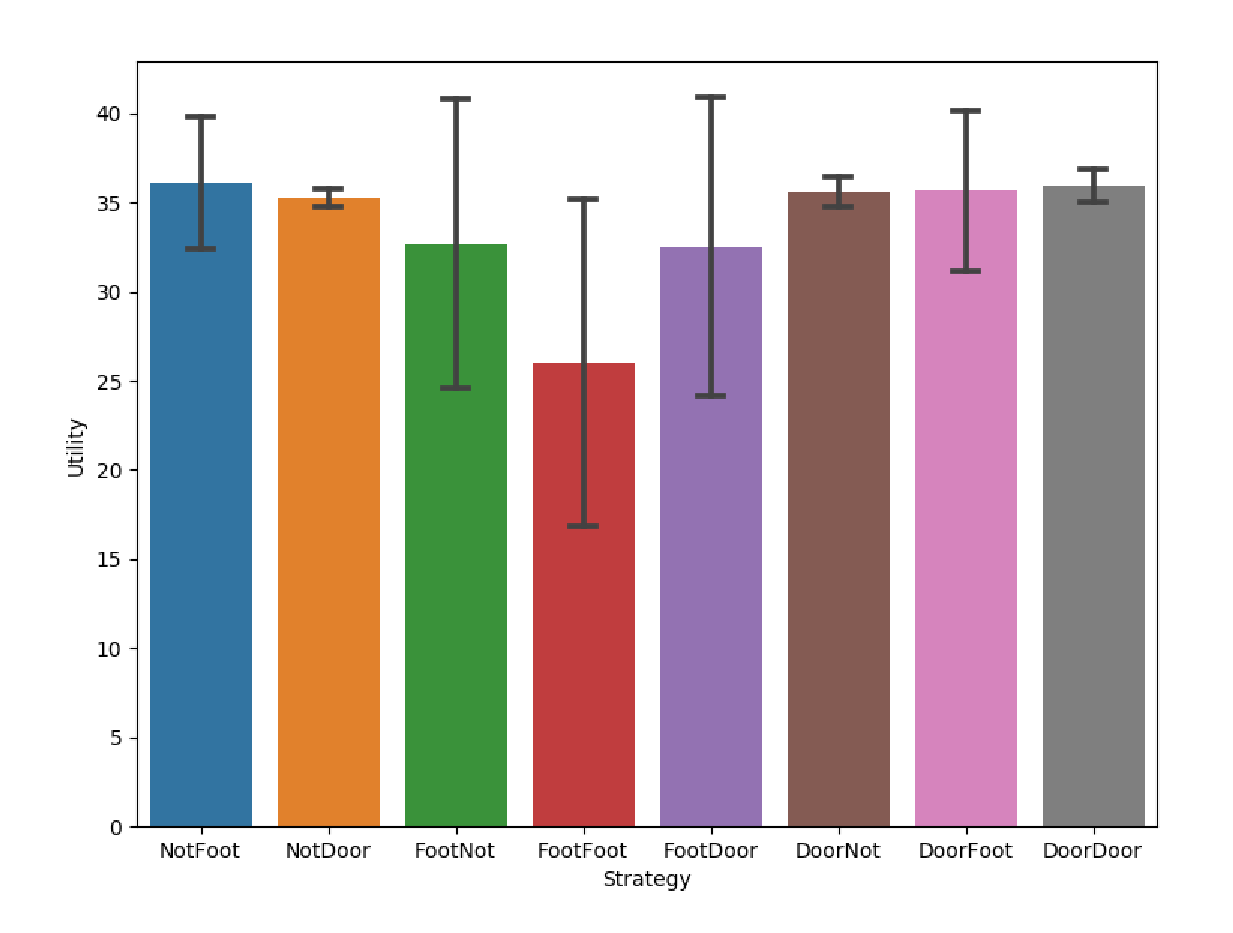
\includegraphics[width=13truecm]{image/bar_utility.eps}
  \caption{提案手法のエージェントの個人効用}
  \label{fig:pre_util}
\end{figure}

\begin{figure}[H]
  \centering
  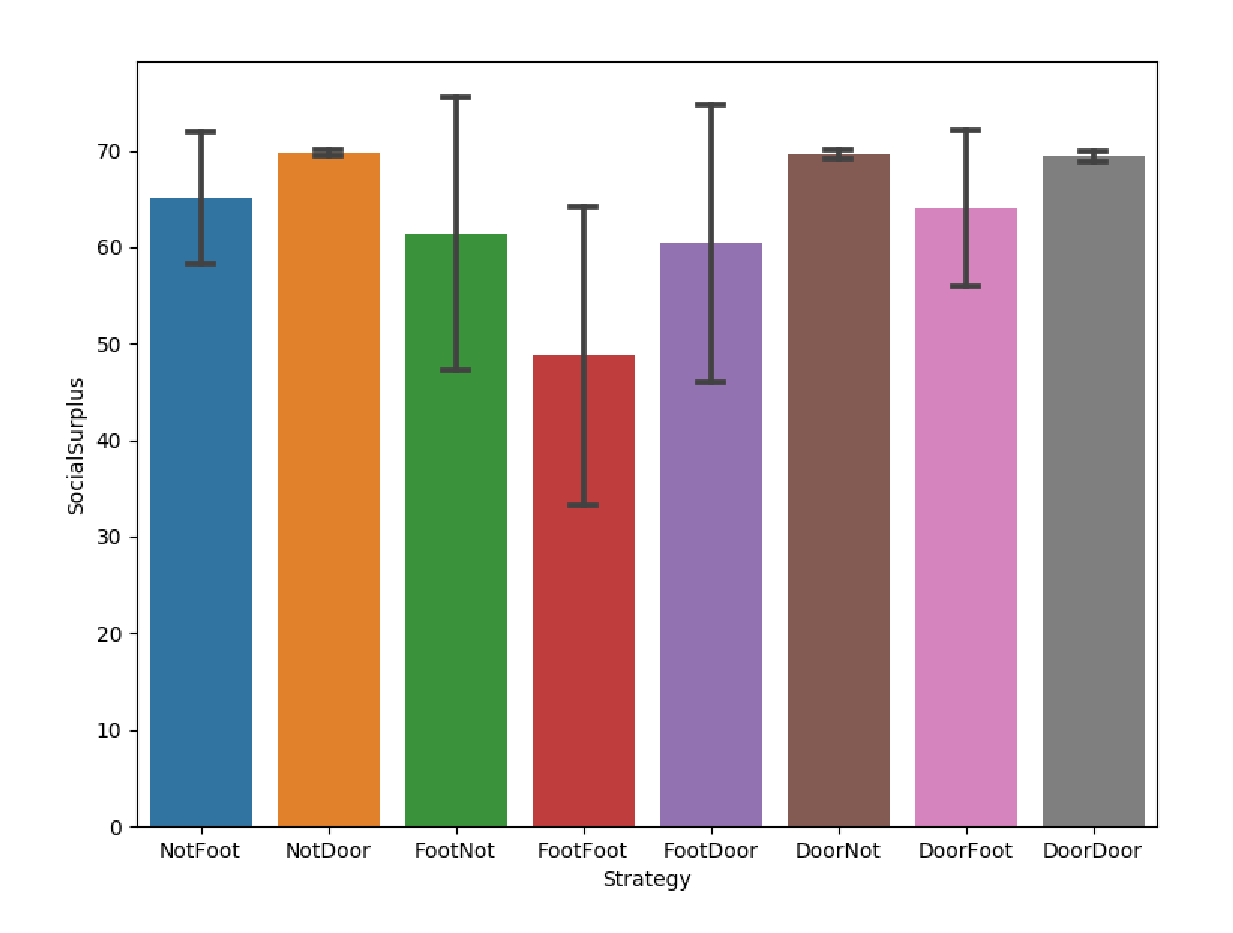
\includegraphics[width=13truecm]{image/bar_social_surplus.eps}
  \caption{エージェントの社会的余剰}
  \label{fig:pre_social}
\end{figure}

\begin{figure}[H]
  \centering
  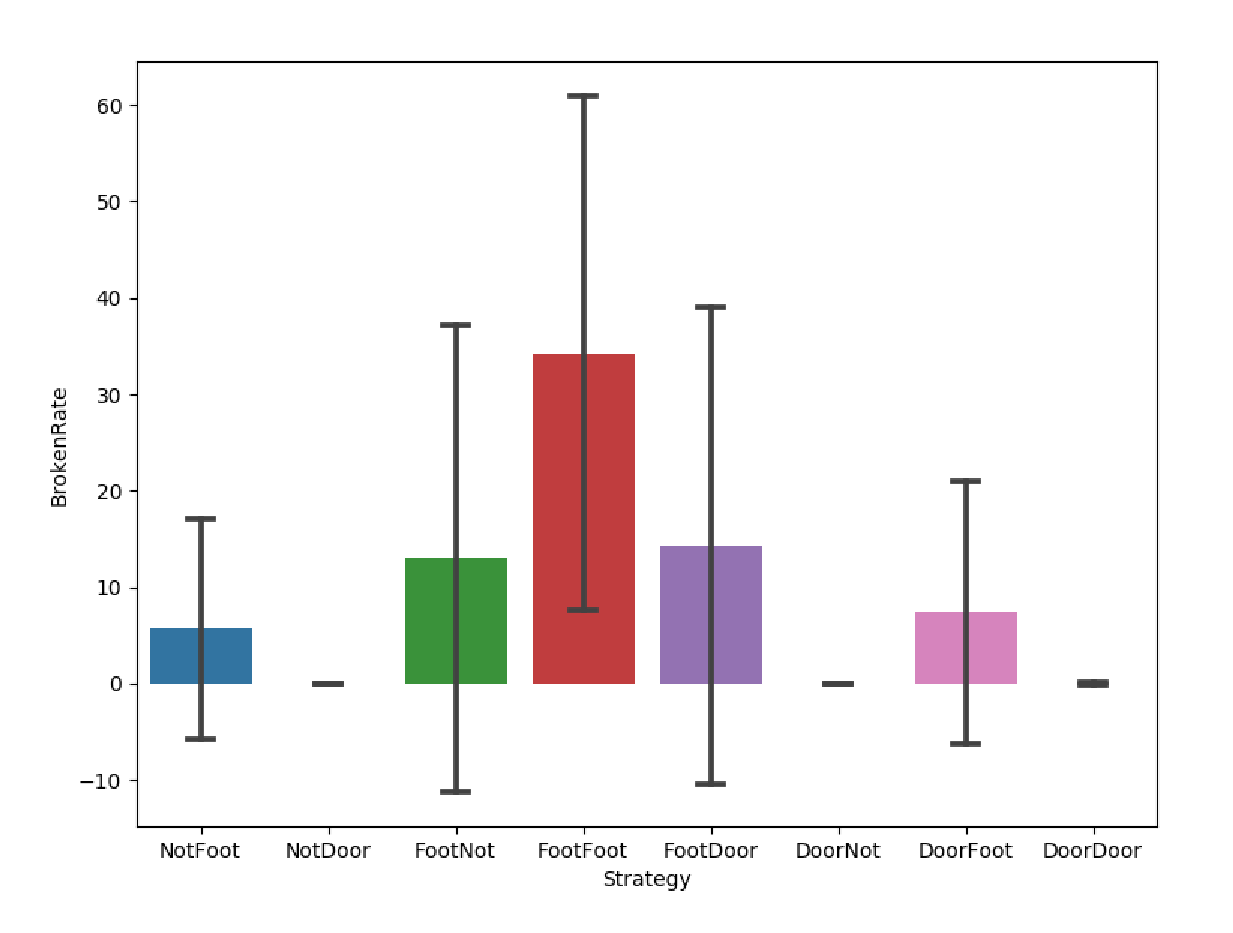
\includegraphics[width=13truecm]{image/bar_broken_rate.eps}
  \caption{提案手法のエージェントの交渉決裂率}
  \label{fig:pre_broken}
\end{figure}


図\ref{fig:pre_broken}のように,FootFootは他の戦略と比較して交渉決裂率の平均値が約$40\%$と高く,一方でNotDoor,DoorNot,DoorDoorは約$0\%$,NotFoot,DoorFootは約$5\%$,FootNot,FootDoorは約$15\%$となった.
FootFootは,相手の提案に対して自らが譲歩することがなく相手の提案を受諾する水準は単調に増加していくため,予備実験用エージェントが譲歩しても合意できない場合が多く交渉決裂率が高くなったと考えられる.FootFootは交渉決裂率が高いため,これに伴って他の戦略と比較してエージェントの個人効用および社会的余剰が低くなってしまったと考えられる.

一方のNotDoor,DoorNot, DoorDoorはいずれも交渉回数および交渉時間に応じて相手の提案を受諾する水準は単調に減少していき,予備実験用エージェントも譲歩していくため最終的にほとんどの交渉において合意に至ったと考えられる.これらの戦略は交渉が決裂することが少なかったため,FootFootと比較してエージェントの効用および社会的余剰が高くなったと考えられる.また,これらの戦略はエージェントの個人効用が平均値が約35,社会的余剰の平均値が約70となっており,分散も小さい.したがって,これらの戦略では安定して社会的余剰が最大となる合意案に達することが可能であると考えられる.

NotFoot,DoorFootはいずれも外側の戦略がFootであり,交渉時間に応じて相手の提案を受諾する水準は単調に増加していくが,内側の戦略では単調減少または変化なしである.そのため,外側の戦略が同じくFootであるFootFootと比較して交渉決裂率が低くなったと考えられる.また,これらの戦略はNotDoor,DoorNot, DoorDoorよりも交渉決裂率が高いにも関わらずエージェントの個人効用の平均値は約35である.したがって,NotFoot,DoorFootの戦略は交渉が合意に至らない可能性があるが代わりに個人効用が高くなりやすい戦略であると考えられる.

FootNot,FootDoorはいずれも内側の戦略がFootであり,交渉回数に応じて相手の提案を受諾する水準は単調に増加していくが,内側の戦略では単調減少または変化なしである.そのため,外側の戦略が同じくFootであるFootFootと比較して交渉決裂率が低くなったと考えられる.また,これらの戦略はNotFoot,DoorFootよりもエージェントの個人効用および社会的余剰の平均値が低くなっている.これは,外側の戦略では4回水準が増加するのに対して,本実験では内側の戦略は平均で5回水準が増加するからであると考えられる.したがって,水準の更新回数が多い内側の戦略にFootを用いているFootNot,FootDoorはNotFoot,DoorFootよりエージェントの個人効用および社会的余剰の平均値が低くなってしまったと考えられる.

\subsection{パラメータ\alpha の実験結果と考察}

予備実験において,パラメータ$\alpha$の増分および初期値ごとの提案手法のエージェントの効用値を図\ref{fig:a_util_1},図\ref{fig:a_util_2},図\ref{fig:a_util_3}に,交渉決裂率を図\ref{fig:a_rate_1},図\ref{fig:a_rate_2},図\ref{fig:a_rate_3}にそれぞれ示す.図\ref{fig:a_util_1},図\ref{fig:a_util_2},図\ref{fig:a_util_3}は縦軸が$\alpha$の増分,横軸が$\alpha$の初期値,色が個人効用を表しており,青に近いほど低い値,赤に近いほど高い値となる.図\ref{fig:a_rate_1},図\ref{fig:a_rate_2},図\ref{fig:a_rate_3}は縦軸が$\alpha$の増分,横軸が$\alpha$の初期値,色が交渉決裂率を表しており,青に近いほど低い値,赤に近いほど高い値となる.

\begin{figure}[H]
  \centering
  \includegraphics[width=15truecm]{image/a_util_1.eps}
  \caption{提案手法のパラメータ$\alpha$における増分・初期値に対する個人効用(1)}
  \label{fig:a_util_1}
\end{figure}

\begin{figure}[H]
  \centering
  \includegraphics[width=15truecm]{image/a_util_2.eps}
  \caption{提案手法のパラメータ$\alpha$における増分・初期値に対する個人効用(2)}
  \label{fig:a_util_2}
\end{figure}

\begin{figure}[H]
  \centering
  \includegraphics[width=15truecm]{image/a_util_3.eps}
  \caption{提案手法のパラメータ$\alpha$における増分・初期値に対する個人効用(3)}
  \label{fig:a_util_3}
\end{figure}

\begin{figure}[H]
  \centering
  \includegraphics[width=15truecm]{image/a_rate_1.eps}
  \caption{提案手法のパラメータ$\alpha$における増分・初期値に対する交渉決裂率(1)}
  \label{fig:a_rate_1}
\end{figure}

\begin{figure}[H]
  \centering
  \includegraphics[width=15truecm]{image/a_rate_2.eps}
  \caption{提案手法のパラメータ$\alpha$における増分・初期値に対する交渉決裂率(2)}
  \label{fig:a_rate_2}
\end{figure}

\begin{figure}[H]
  \centering
  \includegraphics[width=15truecm]{image/a_rate_3.eps}
  \caption{提案手法のパラメータ$\alpha$における増分・初期値に対する交渉決裂率(3)}
  \label{fig:a_rate_3}
\end{figure}

FootNot,FootDoorは$\alpha$の増分が0.5,1.0の場合は$\alpha$の初期値が高くなるにつれて個人効用は高くなり,$\alpha$の増分が1.5以上の場合は$\alpha$の初期値が高くなるにつれて個人効用が低くなった.$\alpha$の増分が低い場合は初期値が高くても相手が譲歩して合意に至ることができたと考えられる.また,$\alpha$の初期値が高い方がエージェントの受諾水準が高くなるため,$\alpha$の増分が低く初期値が高い場合に合意できたときは個人効用が高い値になったと考えられる.一方で,$\alpha$の増分が高い場合は相手が譲歩しても受諾水準が高すぎて合意に至ることができなかったと考えられる.そのため,初期値が高くなるにつれて交渉決裂率が高くなり個人効用が低くなったと考えられる.

FootFootは$\alpha$の増分および初期値が非常に低い場合のみが個人効用が高くなった.FootFootは外側の戦略にもFootを用いているため,$\alpha$の増分および初期値が低い値でないと受諾水準が高くなりすぎてしまうと考えられる.したがって,$\alpha$の増分および初期値が高い場合は交渉決裂率が非常に高くなり,その結果個人効用が低くなると考えられる.一方で,$\alpha$の増分および初期値が非常に低い場合は相手の譲歩を十分に引き出すことができないため,合意に至ったとしても個人効用がFootNot,FootDoorと比較して低くなったと考えられる.

DoorNot,DoorDoorは$\alpha$の初期値が3.0以下のとき$\alpha$の増分に関わらず個人効用はほぼ一定となり,$\alpha$の初期値が4.0以上のときは$\alpha$の増分が低いほど個人効用が高くなった.Door戦略は受諾水準を単調に減少させるため,$\alpha$の初期値が低いと受諾水準が下がりすぎてしまい,合意に至ることはできるが相手の譲歩を引き出すことができず,個人効用が低くなってしまうと考えられる.$\alpha$の初期値が高い場合であっても増分が大きい場合も同様に相手の譲歩を引き出すことができず,個人効用が低くなると考えられる.

DoorFootは$\alpha$の初期値が高く,増分が小さいほど個人効用が低くなった.DoorFootは外側の戦略にFootを用いているため,$\alpha$の初期値が高く,増分が小さい場合は受諾水準が高くなりすぎてしまい,交渉決裂率が上昇し個人効用が低くなると考えられる.それ以外の場合は,個人効用の値および交渉決裂率があまり変化していない.これはDoorNot,DoorDoorと同様の理由で受諾水準が下がりすぎてしまい相手の譲歩を引き出すことができず,個人効用が低くなると考えられる.

また,$\alpha$の更新回数ごとの提案手法のエージェントの個人効用の平均値を図\ref{fig:change_num}に示す.縦軸がエージェントの個人効用,横軸が$\alpha$の更新回数である.

\begin{figure}[H]
  \centering
  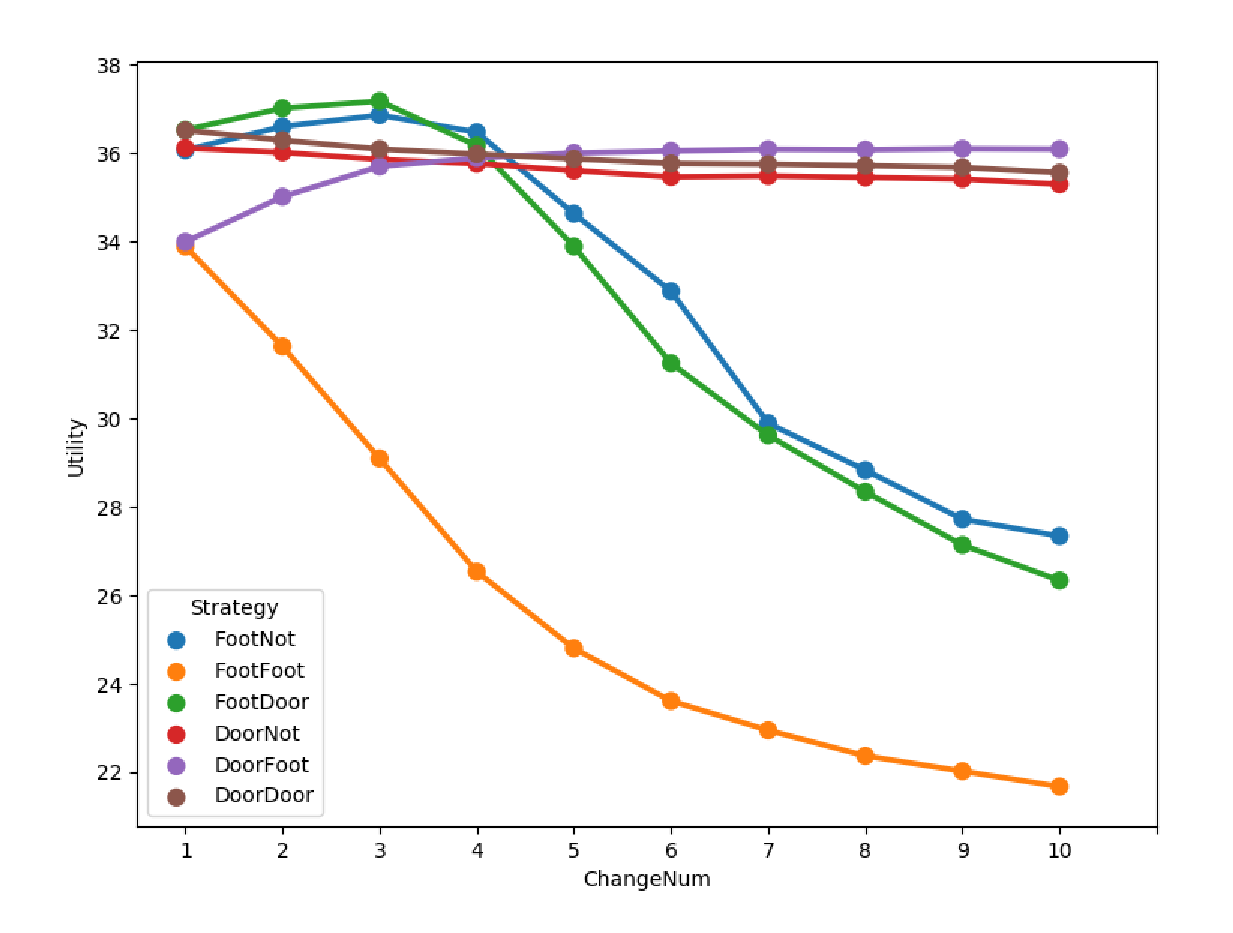
\includegraphics[width=13truecm]{image/change_num.eps}
  \caption{$\alpha$の更新回数に対する個人効用}
  \label{fig:change_num}
\end{figure}

FootNot,FootFoot,FootDoorは他の戦略と比較して$\alpha$の更新回数を変化させた場合の個人効用の変化率が高くなっている.
これらは共通して内側の戦略にFootを用いているため,$\alpha$の更新回数が多いと受諾水準が上昇し,交渉決裂率が上昇するため,個人効用が減少していったと考えられる.一方,DoorNot,DoorDoorは$\alpha$が変化しても個人効用はあまり変化しなかった.これらは内側の戦略にDoorを用いているため,$\alpha$の更新回数が多いと受諾水準が下降し,相手の譲歩が引き出せなくなるが,交渉決裂率は上昇しないため,個人効用の平均値はあまり変化しなかったと考えられる.また,DoorFootは$\alpha$の更新回数が多いほど個人効用が高くなった.DoorFootは外側の戦略がFootであるため,$\alpha$の更新回数が少ない場合,受諾水準が高くなってしまい,交渉決裂率が高くなってしまうと考えられる.

\subsection{パラメータ\beta の実験結果と考察}

予備実験において,パラメータ$\beta$の増分および初期値ごとの提案手法のエージェントの個人効用を図\ref{fig:b_util_1},図\ref{fig:b_util_2},図\ref{fig:b_util_3}に,交渉決裂率を図\ref{fig:b_rate_1},図\ref{fig:b_rate_2},図\ref{fig:b_rate_3}にそれぞれ示す.図\ref{fig:b_util_1},図\ref{fig:b_util_2},図\ref{fig:b_util_3}は縦軸が$\beta$の増分,横軸が$\beta$の初期値,色が個人効用を表しており,青に近いほど低い値,赤に近いほど高い値となる.図\ref{fig:b_rate_1},図\ref{fig:b_rate_2},図\ref{fig:b_rate_3}は縦軸が$\beta$の増分,横軸が$\beta$の初期値,色が交渉決裂率を表しており,青に近いほど低い値,赤に近いほど高い値となる.

\begin{figure}[H]
  \centering
  \includegraphics[width=15truecm]{image/b_util_1.eps}
  \caption{提案手法のパラメータ$\beta$における増分・初期値に対する個人効用(1)}
  \label{fig:b_util_1}
\end{figure}

\begin{figure}[H]
  \centering
  \includegraphics[width=15truecm]{image/b_util_2.eps}
  \caption{提案手法のパラメータ$\beta$における増分・初期値に対する個人効用(2)}
  \label{fig:b_util_2}
\end{figure}

\begin{figure}[H]
  \centering
  \includegraphics[width=15truecm]{image/b_util_3.eps}
  \caption{提案手法のパラメータ$\beta$における増分・初期値に対する個人効用(3)}
  \label{fig:b_util_3}
\end{figure}

\begin{figure}[H]
  \centering
  \includegraphics[width=15truecm]{image/b_rate_1.eps}
  \caption{提案手法のパラメータ$\beta$における増分・初期値に対する交渉決裂率(1)}
  \label{fig:b_rate_1}
\end{figure}

\begin{figure}[H]
  \centering
  \includegraphics[width=15truecm]{image/b_rate_2.eps}
  \caption{提案手法のパラメータ$\beta$における増分・初期値に対する交渉決裂率(2)}
  \label{fig:b_rate_2}
\end{figure}

\begin{figure}[H]
  \centering
  \includegraphics[width=15truecm]{image/b_rate_3.eps}
  \caption{提案手法のパラメータ$\beta$における増分・初期値に対する交渉決裂率(3)}
  \label{fig:b_rate_3}
\end{figure}

NotFoot,DoorFootは$\beta$の増分が1.5から2.0以下の場合は$\beta$の初期値が高くなるにつれて個人効用は高くなり,$\beta$の増分が2.0から2.5以上の場合は$\beta$の初期値が高くなるにつれて個人効用が低くなった.
$\beta$の増分が低い場合は初期値が高くても相手が譲歩して合意に至ることができたと考えられる.
また,$\beta$の初期値が高い方がエージェントの受諾水準が高くなるため,$\beta$の増分が低く初期値が高い場合に合意できたときは個人効用が高い値になったと考えられる.
一方で,$\beta$の増分が高い場合は相手が譲歩しても受諾水準が高すぎて合意に至ることができなかったと考えられる.
そのため,初期値が高くなるにつれて交渉決裂率が高くなり個人効用が低くなったと考えられる.

FootFootは$\beta$の増分および初期値が非常に低い場合のみが個人効用が高くなった.
FootFootは内側の戦略にもFootを用いているため,$\beta$の増分および初期値が低い値でないと受諾水準が高くなりすぎてしまうと考えられる.したがって,$\beta$の増分および初期値が高い場合は交渉決裂率が非常に高くなり,その結果個人効用が低くなると考えられる.一方で,$\beta$の増分および初期値が非常に低い場合は相手の譲歩を十分に引き出すことができないため,合意に至ったとしても個人効用がNotFoot,DoorFootと比較して低くなったと考えられる.

NotDoor,DoorDoorは$\beta$の初期値が3.0以下のとき$\beta$の増分に関わらず個人効用はほぼ一定となり,
$\beta$の初期値が4.0以上のときは$\beta$の増分が低いほど個人効用が高くなった.Door戦略は受諾水準を単調に減少させるため,$\beta$の初期値が低いと受諾水準が下がりすぎてしまい,合意に至ることはできるが相手の譲歩を引き出すことができず,個人効用が低くなってしまうと考えられる.$\beta$の初期値が高い場合であっても増分が大きい場合も同様に相手の譲歩を引き出すことができず,個人効用が低くなると考えられる.

FootDoorは$\beta$の初期値が高く,増分が小さいほど個人効用が低くなった.
FootDoorは内側の戦略にFootを用いているため,$\beta$の初期値が高く,増分が小さい場合は受諾水準が高くなりすぎてしまい,交渉決裂率が上昇し個人効用が低くなると考えられる.それ以外の場合は,個人効用の値および交渉決裂率があまり変化していない.これはNotDoor,DoorDoorと同様の理由で受諾水準が下がりすぎてしまい相手の譲歩を引き出すことができず,個人効用が低くなると考えられる.また,図\ref{fig:b_util_2}は全体的に効用の平均値があまり変化していないのに対して図\ref{fig:a_util_2}は効用の値はばらつきが大きい.このことから,FootDoorに関しては内側のパラメータによって個人効用が大きく左右されると考えられる.

\section{実験のまとめ}
予備実験の結果をまとめると以下のようになる.
\begin{itemize}
  \item Foot戦略において初期値および増分の値を高く設定すると個人効用が低くなる.
  \item Door戦略において初期値を高く,増分を低く設定すると個人効用が高くなる.
  \item 交渉決裂率はFootFootが最も高い.
\end{itemize}


%内容ここまで

\chapter*{謝辞}
本論文を執筆するにあたり,多数の方々からご指導・ご協力いただきましたことを,心より御礼申し上げます.

指導教員である藤田桂英准教授には,研究の機会を与えていただき,研究の方針に関する助言や発表練習等の
多大なるご指導や助言をいただきましたことを深く感謝いたします.

研究に関する知識のご教示に加えて,本実験の準備を行うにあたってWEBサーバを構築する際にお力添えいただいた松根鷹生様に深く感謝申し上げます.
また,藤田桂英研究室の皆様には研究に必要な知識や意見等をいただいたことを心より感謝いたします.

本実験を行うにあたってお忙しい中ご協力いただいた同期の編入生の方々,および安井貴規様がいなければ本論文は完成に至りませんでした.
心より御礼申し上げます.

最後に,様々な面で私を支えていただいた家族に,心より感謝いたします.ありがとうございました.

\bibliographystyle{plain}
\bibliography{reference}


\begin{comment}
%付録で発表論文をつけてアピールだ!!

\renewcommand{\bibname}{付録 発表論文一覧}
%\chapter{発表論文一覧}

\begin{thebibliography}{99}
\item S. Kakimoto and K. Fujita. 二者間複数論点交渉問題におけるパレートフロント推定手法の提案. Joint Agent Workshop and Symposium, 2014.
\item S. Kakimoto and K. Fujita. Estimating Pareto Fronts using Interdependency between Issues for Bilateral Multi-issue Closed Nonlinear Negotiations. Applications Knowledge and Service Technology for Life, Environment, and Sustainability workshop(KASTLES),2014.
\item S. Kakimoto and K. Fujita. 二者間非線形交渉問題におけるパレートフロント推定を利用した自動交渉エージェントの設計と評価. 情報処理学会 第177回 知能システム研究会, 2014.

\end{thebibliography}

\end{comment}

\end{document}


\documentclass[a4paper, 10.5pt, twoside]{jreport}

% include
\usepackage{gra_yasuda}
\usepackage{lscape}
\usepackage{graphicx}
\usepackage{here}
\usepackage{color}
\usepackage{amsmath}
\usepackage{subfig}
\usepackage{tascmac}
\usepackage{url}
\usepackage{ascmac}
\usepackage{booktabs}
\usepackage{otf}
\usepackage{comment}



%タイトル
\title{心理的効果を用いた人間とエージェントの繰り返し交渉戦略}
\etitle{Repetitive negotiation strategy of human and agent \\ using psychological effect}

%名前
\author{松下 昌悟}
\eauthor{Shogo MATSUSHITA}

%入学年度
\enteryear{2017}
%卒業年度
\graduateyear{2018}

%学籍番号
\studentnumber{17268508}

%提出日
\date{平成30年1月31日}

\begin{document}

%ここで行ピッチを指定
%フォントを変えるとサイズがリセットされてしまうので注意
\setlength{\baselineskip}{8truemm}


%ここから内容

% Chapter 5
\chapter{評価実験}\label{cha:5}

\section{目的と概要}
提案手法の有用性を示すことを目的として人間とエージェントで交渉を行う.
被験者は提案手法の戦略を適用した8つのエージェントにベースラインであるNotNotエージェントを加えた計9種類のエージェント全てと交渉を行う.
本実験では,提案手法の戦略を適用したエージェントの個人効用が高いほど良い戦略であると評価する.

\section{実験設定}
評価実験では,予備実験と同様に各論点が$0\sim 5$の計6つの選択肢を有する,4つの論点について交渉を行う.
評価実験で用いるドメインは予備実験で用いたドメイン(表\ref{tab:pre_domain})と同一のものである.
各論点の価値は交渉ごとに毎回ランダムで変化し,エージェントと被験者の各論点の価値の関係は予備実験と同様であり,社会的余剰の最大値は70である.
1交渉300秒とし,被験者はチュートリアルとして1回交渉を行なったのちに,各エージェントと5回連続で交渉を行う.
被験者,エージェントは自分にとっての各論点の価値のみを知っており,相手にとっての価値はわからない状態から交渉が開始する.
相手にとっての価値は相手の選好に関する返答や相手の提案内容から予想する.
本実験は9人の被験者に対して行なった.被験者ごとに交渉するエージェントの順番は異なり,ラテン方格法によって決定した.
交渉中,被験者は以下の行動を取ることができる.
\begin{enumerate}
  \renewcommand{\labelenumi}{(\arabic{enumi}).}
  \item 自分の選好の相対的な関係を1つ相手に伝える
  \item 相手の選好について質問する
  \item 自分の感情を相手に伝える
  \item 相手に固定メッセージを送信する
  \item エージェントに提案を行う
  \item エージェントから送られてきた提案を受諾もしくは拒否する
  \item 被験者にとっての各論点の価値を確認する
\end{enumerate}
交渉はエージェントと被験者の両者がFullOfferを受諾するか交渉の残り時間が0になると終了する.
基本的にエージェントは被験者の行動に対して受動的に行動する.
例として,被験者が(1)の行動を行うとエージェントは自分の選好の相対的な関係を1つ被験者に伝える.
他の被験者の行動に対しても同様である.
エージェントが被験者に対して能動的に提案を行うのは交渉の残り時間が30秒となったとき,被験者がエージェントに提案を要求する固定メッセージを送信したときのみである.同様にエージェントから新しい提案を行うことはなく,被験者から送信された提案を拒否した場合に提案を行う.
予備実験をもとに戦略ごとに決定したパラメータを表\ref{tab:eva_para}に示す.被験者はこれらのエージェントと交渉を行う.

\begin{table}[htb]
  \begin{center}
    \caption{評価実験で用いるパラメータ}
    \label{tab:eva_para}
    \begin{tabular}{|c|c|c|c|c|c|} \hline
      & \alpha の初期値 & \alpha の増分 & \beta の初期値 & \beta の増分 & \alpha の更新回数 \\ \hline \hline
      NotNot & 0.0 & 0.0 & 0.0 & 0.0 & 0 \\ \hline
      NotFoot & 0.0 & 0.0 & 8.0 & 0.5 & 0 \\ \hline
      NotDoor & 0.0 & 0.0 & 8.0 & 0.5 & 0 \\ \hline
      FootNot & 8.0 & 0.5 & 0.0 & 0.0 & 3 \\ \hline
      FootFoot & 0.0 & 0.5 & 0.0 & 0.5 & 1 \\ \hline
      FootDoor & 8.0 & 2.0 & 0.5 & 1.0 & 3 \\ \hline
      DoorNot & 8.0 & 0.5 & 0.0 & 0.0 & 1 \\ \hline
      DoorFoot & 2.0 & 1.0 & 8.0 & 0.5 & 10 \\ \hline
      DoorDoor & 8.0 & 0.5 & 8.0 & 0.5 & 1 \\ \hline
    \end{tabular}
  \end{center}
\end{table}

\section{実験結果と考察}
エージェントの個人効用の平均とその分散,被験者の個人効用の平均とその分散,エージェントと被験者の個人効用の差分の平均とその分散,エージェントと被験者の社会的余剰の平均とその分散,エージェントの交渉決裂率の平均とその分散をそれぞれ図\ref{fig:res_util_vh},図\ref{fig:res_util_user},図\ref{fig:res_util_diff},図\ref{fig:res_social},図\ref{fig:res_broken}に示す.

\begin{figure}[H]
  \centering
  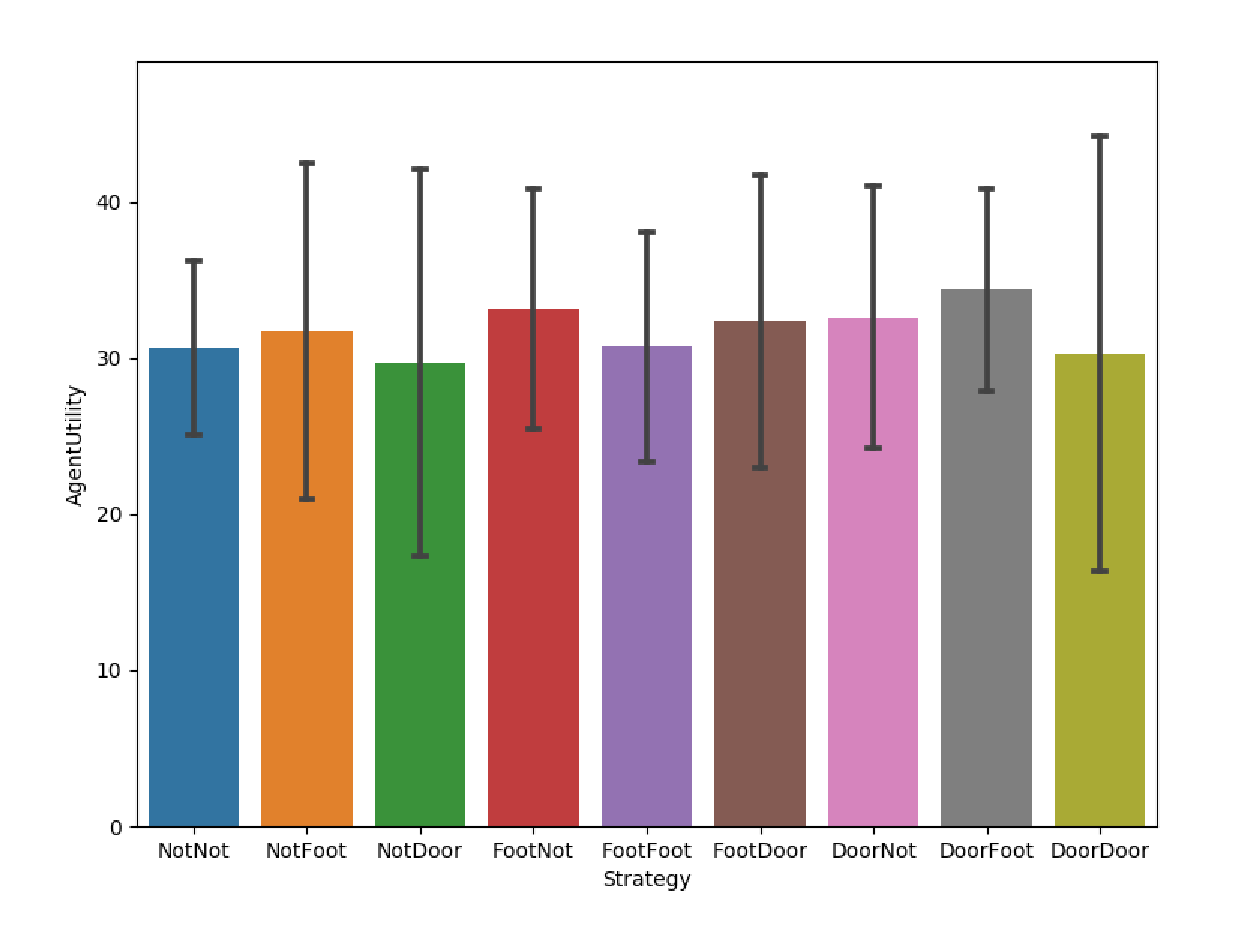
\includegraphics[width=12truecm]{image/util_vh.eps}
  \caption{エージェントの個人効用}
  \label{fig:res_util_vh}
\end{figure}

\begin{figure}[H]
  \centering
  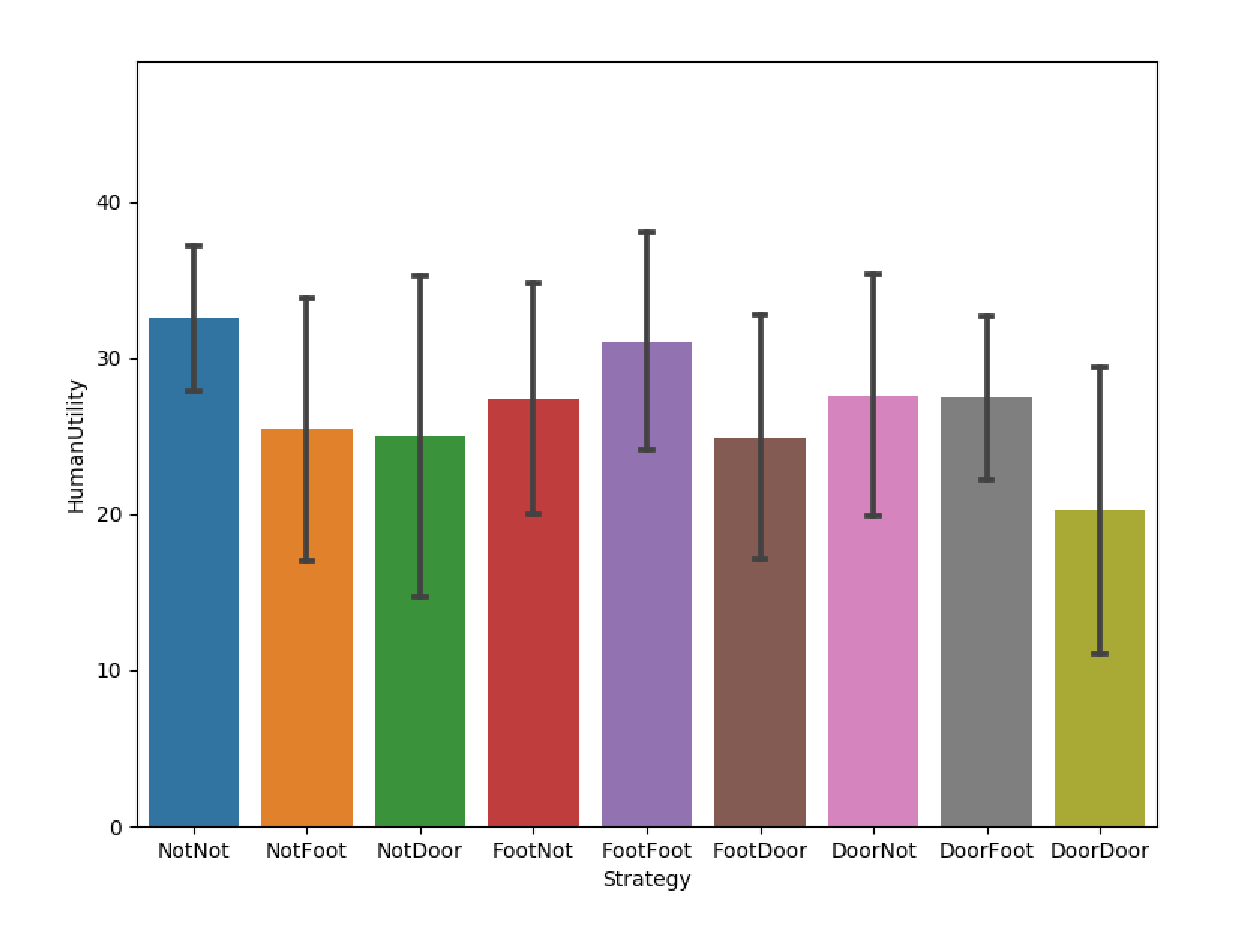
\includegraphics[width=12truecm]{image/util_user.eps}
  \caption{被験者の個人効用}
  \label{fig:res_util_user}
\end{figure}

\begin{figure}[H]
  \centering
  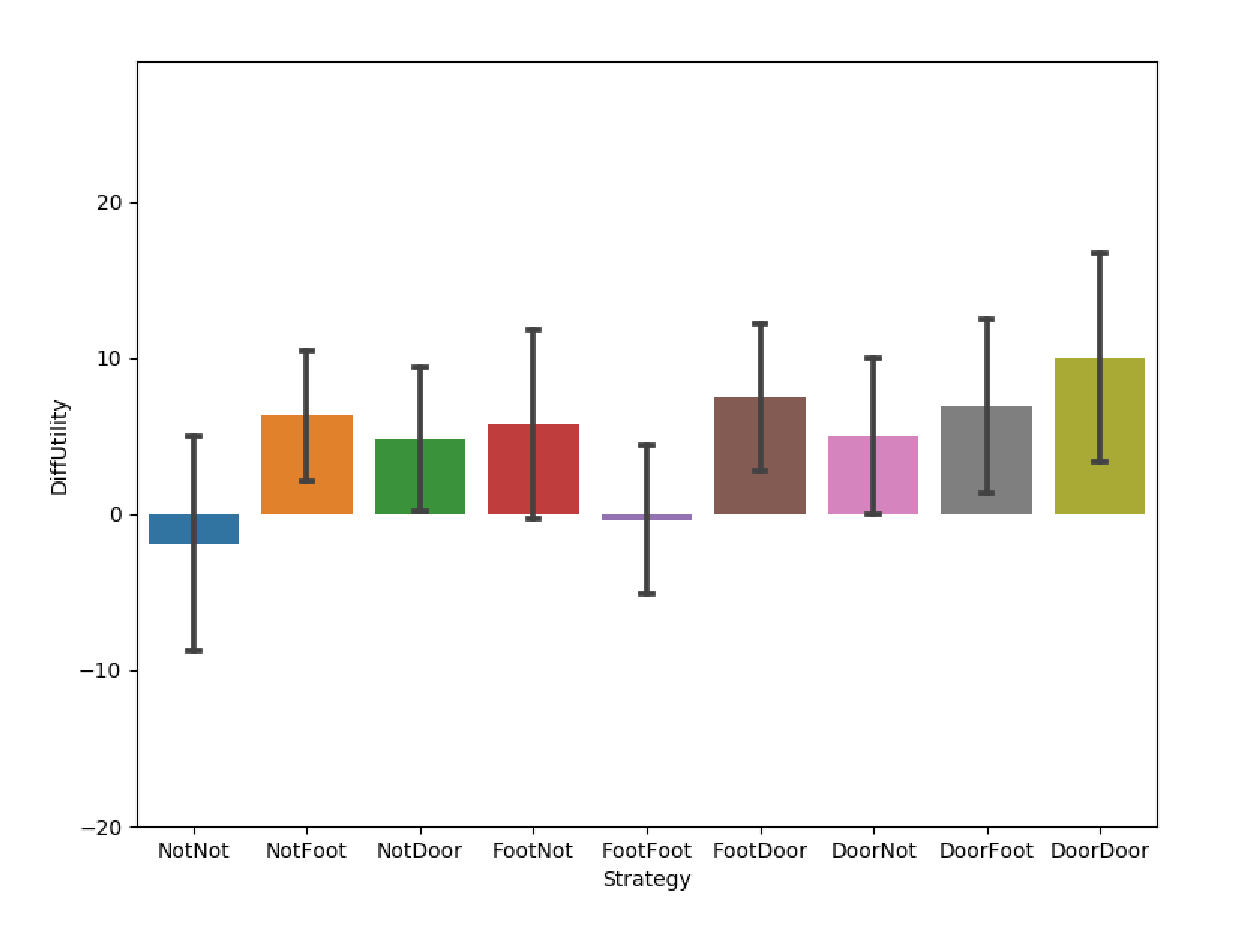
\includegraphics[width=12truecm]{image/result_utility_diff.eps}
  \caption{エージェントと被験者の個人効用の差分}
  \label{fig:res_util_diff}
\end{figure}

\begin{figure}[H]
  \centering
  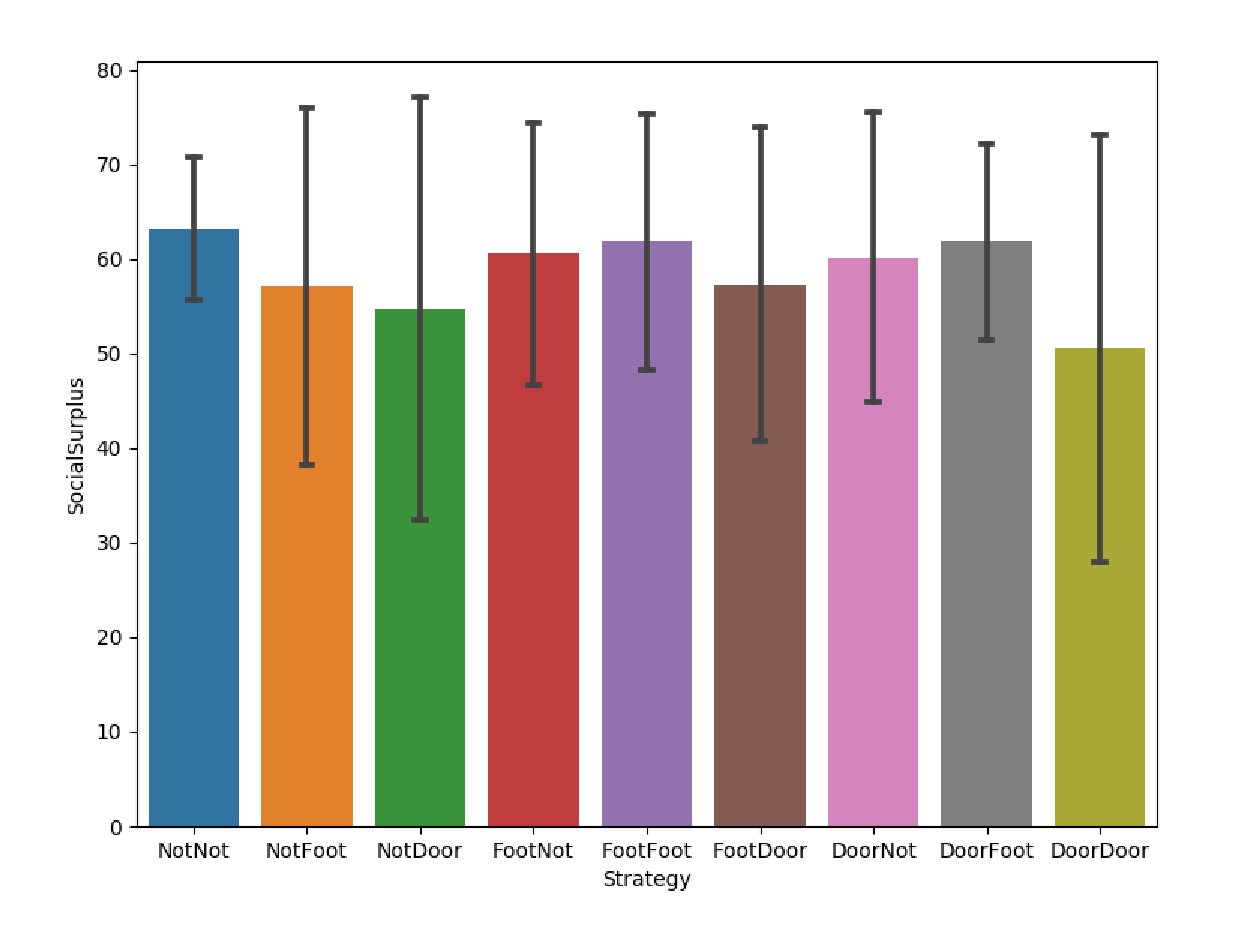
\includegraphics[width=12truecm]{image/result_social_surplus.eps}
  \caption{エージェントと被験者の社会的余剰}
  \label{fig:res_social}
\end{figure}

\begin{figure}[H]
  \centering
  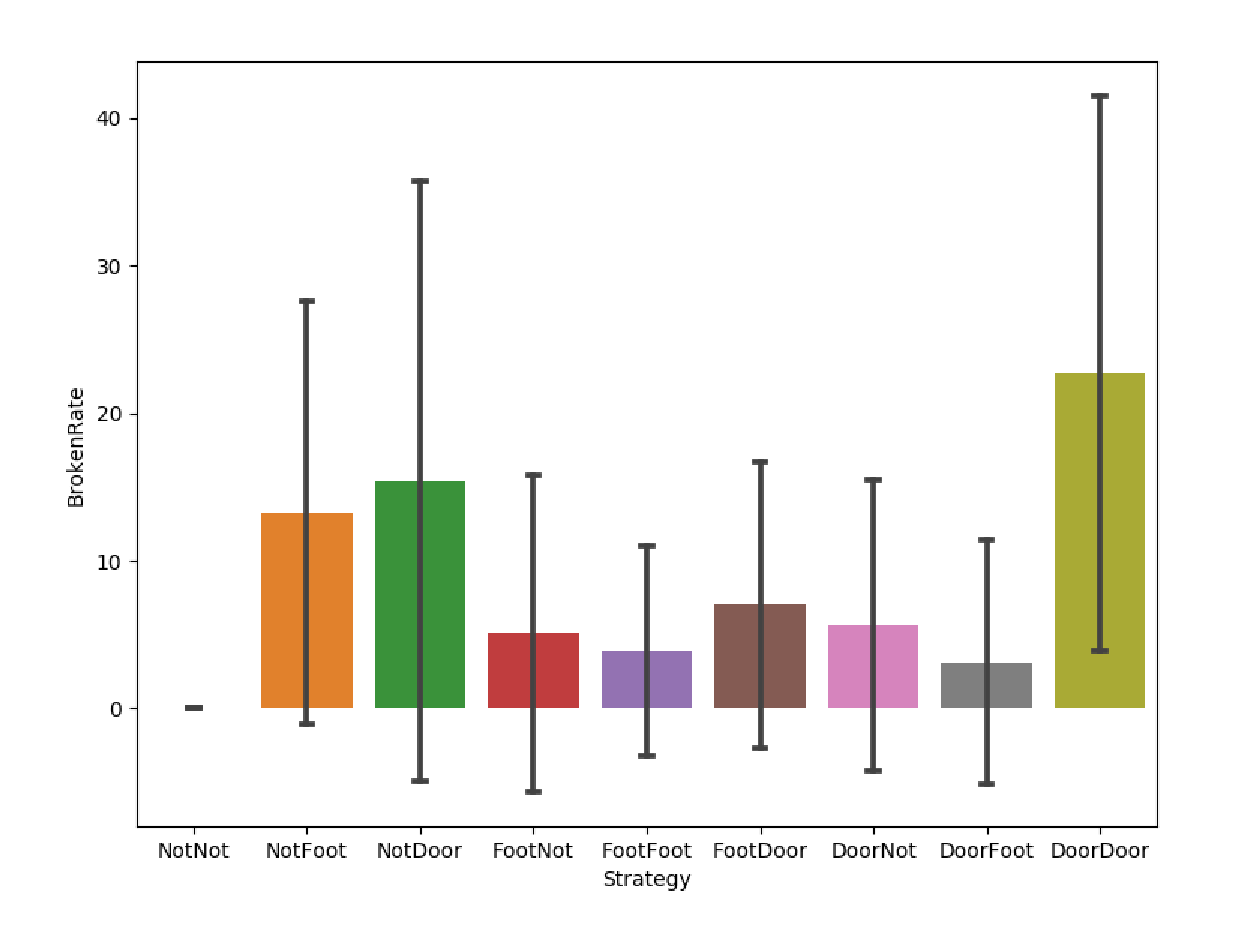
\includegraphics[width=12truecm]{image/result_broken_rate.eps}
  \caption{エージェントの交渉決裂率}
  \label{fig:res_broken}
\end{figure}

NotNot,FootFoot以外の戦略では被験者よりエージェントの方が個人効用が高くなった,NotNotとFootFootは社会的余剰も高いため,他の戦略と比較するとエージェントと被験者が公平な提案で合意したと考えられる.今回,FootFootは$\alpha$および$\beta$の増分が小さく.$\alpha$の更新回数も1回であるので,受諾水準がNotNotとあまり変わらなかったためNotNotと類似した結果となったと考えられる.

DoorDoorは被験者とエージェントの個人効用の差が最大となった.DoorDoorは$\alpha$および$\beta$の初期値が高く,増分が小さいので受諾水準が高いため,合意に至った場合はエージェントが被験者より個人効用が高くなるが,交渉決裂率も全戦略の中で最も高いため,エージェントおよび被験者の効用,社会的余剰が最も低くなったと考えられる.

外側にDoorを用いているNotDoor,FootDoor,DoorDoorはいずれも被験者の個人効用が低く,社会的余剰も低くなった.予備実験におけるDoorの結果を踏まえ,評価実験では$\beta$の初期値を高く,増分を低い値に設定したためエージェントの受諾水準が高くなり,合意に至っても被験者の効用が低くなったと考えられる.

NotFoot,FootNotは片側にFoot,もう片側にNotを用いた戦略であり,パラメータの初期値,増分も同じ値であるにも関わらず交渉決裂率の平均がNotFootの方がFootNotと比較して$10\%$程度高くなっている.また,同様にNotDoor,DoorNotも同様の傾向が見られる.このことから,外側戦略の方が被験者に与える影響が大きくなると考えられる.

予備実験の結果と比較するとほとんどの戦略で社会的余剰,個人効用ともに減少している.予備実験ではエージェント同士で交渉を行い,パラメータを設定したため,人間との交渉においては適していないパラメータになっていたため,個人効用が低下したと考えられる.また,Doorを用いた戦略は初期値が高く,増分が低いパラメータを設定したため,交渉決裂率が高い戦略が多かった.また,合意に至った場合でも個人効用の差が大きいため,公平な提案で合意が行えておらず,良好な関係構築は果たせていないと考えられる.9種類のエージェントの中でNotNotだけが唯一交渉決裂率が$0\%$となった.他の戦略は全てNotNotよりも受諾水準が高いため,これに伴って交渉が決率する回数も多くなっていったと考えられる.

\section{実験のまとめ}
評価実験の結果をまとめると以下のようになる.
\begin{itemize}
  \item 全ての戦略でNotNotより個人効用の差が大きくなった.
  \item DoorDoor戦略は個人効用の差は最も大きくなったが,社会的余剰,被験者とエージェントの個人効用は最も小さくなった.
  \item 社会的余剰はNotNotよりも低い戦略が多く,良好な関係を構築できているとは言い難い.
\end{itemize}

%内容ここまで

\chapter*{謝辞}
本論文を執筆するにあたり,多数の方々からご指導・ご協力いただきましたことを,心より御礼申し上げます.

指導教員である藤田桂英准教授には,研究の機会を与えていただき,研究の方針に関する助言や発表練習等の
多大なるご指導や助言をいただきましたことを深く感謝いたします.

研究に関する知識のご教示に加えて,本実験の準備を行うにあたってWEBサーバを構築する際にお力添えいただいた松根鷹生様に深く感謝申し上げます.
また,藤田桂英研究室の皆様には研究に必要な知識や意見等をいただいたことを心より感謝いたします.

本実験を行うにあたってお忙しい中ご協力いただいた同期の編入生の方々,および安井貴規様がいなければ本論文は完成に至りませんでした.
心より御礼申し上げます.

最後に,様々な面で私を支えていただいた家族に,心より感謝いたします.ありがとうございました.

\bibliographystyle{plain}
\bibliography{reference}


\begin{comment}
%付録で発表論文をつけてアピールだ!!

\renewcommand{\bibname}{付録 発表論文一覧}
%\chapter{発表論文一覧}

\begin{thebibliography}{99}
\item S. Kakimoto and K. Fujita. 二者間複数論点交渉問題におけるパレートフロント推定手法の提案. Joint Agent Workshop and Symposium, 2014.
\item S. Kakimoto and K. Fujita. Estimating Pareto Fronts using Interdependency between Issues for Bilateral Multi-issue Closed Nonlinear Negotiations. Applications Knowledge and Service Technology for Life, Environment, and Sustainability workshop(KASTLES),2014.
\item S. Kakimoto and K. Fujita. 二者間非線形交渉問題におけるパレートフロント推定を利用した自動交渉エージェントの設計と評価. 情報処理学会 第177回 知能システム研究会, 2014.

\end{thebibliography}

\end{comment}

\end{document}


\documentclass[a4paper, 10.5pt, twoside]{jreport}

% include
\usepackage{gra_yasuda}
\usepackage{lscape}
\usepackage{graphicx}
\usepackage{here}
\usepackage{color}
\usepackage{amsmath}
\usepackage{subfig}
\usepackage{tascmac}
\usepackage{url}
\usepackage{ascmac}
\usepackage{booktabs}
\usepackage{otf}
\usepackage{comment}



%タイトル
\title{心理的効果を用いた人間とエージェントの繰り返し交渉戦略}
\etitle{Repetitive negotiation strategy of human and agent \\ using psychological effect}

%名前
\author{松下 昌悟}
\eauthor{Shogo MATSUSHITA}

%入学年度
\enteryear{2017}
%卒業年度
\graduateyear{2018}

%学籍番号
\studentnumber{17268508}

%提出日
\date{平成30年1月31日}

\begin{document}

%ここで行ピッチを指定
%フォントを変えるとサイズがリセットされてしまうので注意
\setlength{\baselineskip}{8truemm}


%ここから内容

% Chapter 6
\chapter{おわりに}\label{cha:6}
\section{まとめ}
本研究では,同じ相手と繰り返し交渉する場合に適応可能な戦略として,段階的要請法,譲歩的要請法を組み合わせて受諾水準を変化させる戦略を提案した.
提案した戦略をIAGOのPinocchioエージェントに適応させたエージェントを作成し,エージェントのパラメータを決定するために予備実験を行なった.

予備実験を行なった結果,Foot戦略において初期値および増分の値を高く設定すると個人効用が低くなり,Door戦略において初期値を高く,増分を低く設定すると個人効用が高くなる傾向があることが確認できた.
また,予備実験で決定したパラメータを設定したエージェントを用いて被験者に対して評価実験を行なった.
評価実験を行なった結果,提案した戦略全てが繰り返し交渉に対応していないNotNotより個人効用の差が大きくなったが,
社会的余剰はNotNotよりも低い戦略が多く,良好な関係を構築できていないことが確認できた.

\section{今後の課題}
\begin{description}
  \item[人間との関係構築に関する課題]~\\
  今回の戦略では受諾水準を変化させることで個人効用を上昇させたが,交渉が決裂するよりは公平でなくても提案を受諾した方が良いため仕方なく合意に至ったというケースが多く,両者が歩み寄るような良好な関係を構築できたとは言い難い.関係構築がうまくいかない場合,同じ相手と交渉をするときに不利益を被ってしまうため,良好な関係を保ちつつ個人効用を上昇させるような繰り返し交渉戦略を提案する必要がある.
  \item[パラメータの値に関する課題]~\\
  予備実験ではエージェント同士で交渉を行うことで評価実験に用いるパラメータを決定した.しかし,評価実験では人間とエージェントが交渉を行うため,パラメータの値が最適な値でない可能性がある.そのため,パラメータの調整も含めて人間とエージェントで交渉を行うことでより良い結果になる可能性がある.
  \item[受諾水準の変化に関する課題]~\\
  本稿では受諾水準を時間経過,交渉回数の2種類で変化させた.時間経過による変化はステップ関数的に,交渉回数による変化は線形関数的に変化させたが,これらを対数関数など他の関数を用いて変化させることで人間の譲歩をより再現することができ,社会的余剰を高めつつ個人効用を高めることができる可能性がある.
  \item[被験者数による実験結果の誤差に関する課題]~\\
  評価実験では9人の被験者に対して実験を行なった.エージェントと交渉する順番による順序効果を相殺するために$9n$人に対して実験を行う必要があり,本稿では$n = 1$として実験を行なった.しかし,$n = 1$では各個人の誤差が結果に反映されてしまい,結果が正しくない可能性がある.したがって,$n$の値を大きくして実験を行う必要がある.
\end{description}


%内容ここまで

\chapter*{謝辞}
本論文を執筆するにあたり,多数の方々からご指導・ご協力いただきましたことを,心より御礼申し上げます.

指導教員である藤田桂英准教授には,研究の機会を与えていただき,研究の方針に関する助言や発表練習等の
多大なるご指導や助言をいただきましたことを深く感謝いたします.

研究に関する知識のご教示に加えて,本実験の準備を行うにあたってWEBサーバを構築する際にお力添えいただいた松根鷹生様に深く感謝申し上げます.
また,藤田桂英研究室の皆様には研究に必要な知識や意見等をいただいたことを心より感謝いたします.

本実験を行うにあたってお忙しい中ご協力いただいた同期の編入生の方々,および安井貴規様がいなければ本論文は完成に至りませんでした.
心より御礼申し上げます.

最後に,様々な面で私を支えていただいた家族に,心より感謝いたします.ありがとうございました.

\bibliographystyle{plain}
\bibliography{reference}


\begin{comment}
%付録で発表論文をつけてアピールだ!!

\renewcommand{\bibname}{付録 発表論文一覧}
%\chapter{発表論文一覧}

\begin{thebibliography}{99}
\item S. Kakimoto and K. Fujita. 二者間複数論点交渉問題におけるパレートフロント推定手法の提案. Joint Agent Workshop and Symposium, 2014.
\item S. Kakimoto and K. Fujita. Estimating Pareto Fronts using Interdependency between Issues for Bilateral Multi-issue Closed Nonlinear Negotiations. Applications Knowledge and Service Technology for Life, Environment, and Sustainability workshop(KASTLES),2014.
\item S. Kakimoto and K. Fujita. 二者間非線形交渉問題におけるパレートフロント推定を利用した自動交渉エージェントの設計と評価. 情報処理学会 第177回 知能システム研究会, 2014.

\end{thebibliography}

\end{comment}

\end{document}



%ここまで

\chapter*{謝辞}
本論文を執筆するにあたり,多数の方々からご指導・ご協力いただきましたことを,心より御礼申し上げます.

指導教員である藤田桂英准教授には,研究の機会を与えていただき,研究の方針に関する助言や発表練習等の
多大なるご指導や助言をいただきましたことを深く感謝いたします.

研究に関する知識のご教示に加えて,本実験の準備を行うにあたってWEBサーバを構築する際にお力添えいただいた松根鷹生様に深く感謝申し上げます.
また,藤田桂英研究室の皆様には研究に必要な知識や意見等をいただいたことを心より感謝いたします.

本実験を行うにあたってお忙しい中ご協力いただいた同期の編入生の方々,および安井貴規様がいなければ本論文は完成に至りませんでした.
心より御礼申し上げます.

最後に,様々な面で私を支えていただいた家族に,心より感謝いたします.ありがとうございました.

\bibliographystyle{plain}
\bibliography{reference}


\begin{comment}
%付録で発表論文をつけてアピールだ!!

\renewcommand{\bibname}{付録 発表論文一覧}
%\chapter{発表論文一覧}

\begin{thebibliography}{99}
\item S. Kakimoto and K. Fujita. 二者間複数論点交渉問題におけるパレートフロント推定手法の提案. Joint Agent Workshop and Symposium, 2014.
\item S. Kakimoto and K. Fujita. Estimating Pareto Fronts using Interdependency between Issues for Bilateral Multi-issue Closed Nonlinear Negotiations. Applications Knowledge and Service Technology for Life, Environment, and Sustainability workshop(KASTLES),2014.
\item S. Kakimoto and K. Fujita. 二者間非線形交渉問題におけるパレートフロント推定を利用した自動交渉エージェントの設計と評価. 情報処理学会 第177回 知能システム研究会, 2014.

\end{thebibliography}

\end{comment}

\end{document}

